\documentclass[11pt]{sig-alternate}
\usepackage{hyperref}
\usepackage{tabularx}
\usepackage{graphicx}
\usepackage{blindtext}
\usepackage[utf8]{inputenc}
\usepackage[english]{babel}
\usepackage{lastpage}
\usepackage{comment}
\usepackage{dirtytalk}
\usepackage{xcolor}
\usepackage{hanging}
\usepackage{wrapfig}
\usepackage[backend=biber, style=apa]{biblatex}
\addbibresource{notation.bib}
\usepackage{authblk}
\usepackage{caption}
\usepackage{subcaption}
\usepackage{graphicx,subfigure}
\usepackage{authblk}
\usepackage{enumitem}
\usepackage[utf8]{inputenc}
\usepackage{cuted}
\usepackage{fancyhdr}
\usepackage{xurl}
\usepackage{longtable}
\pagestyle{fancy}
\renewcommand{\headrulewidth}{0pt}
\renewcommand{\footrulewidth}{0pt}
\setlength\headheight{80.0pt}
\addtolength{\textheight}{-80.0pt}
\chead{%
  \ifcase\value{page}
  % empty test for page = 0
  \or 
\includegraphics[width=\textwidth]{headerImage.png}% page=1
  \or 
\includegraphics[width=\textwidth]{headerImage.png}% page = 2
  \or 
\includegraphics[width=\textwidth]{headerImage.png}% page = 3
  \or 
\includegraphics[width=\textwidth]{headerImage.png}% page = 4
  \or 
\includegraphics[width=\textwidth]{headerImage.png}% page = 5
  \else
  
\includegraphics[width=\textwidth]{headerImage.png}
  \fi
}
%\chead{
\includegraphics[width=\textwidth]{headerImage.png}}
\fancyfoot[LE,LO]{STEM and high school students with disabilities: A qualitative review of the research literature\\           
DOI: 10.14448/jsesd.13.0006}
\fancyfoot[CE,CO]{{ }}
\fancyfoot[RE,RO]{\thepage}
\pagenumbering{arabic}
\hypersetup{
    colorlinks=true,
    urlcolor=blue
}
 
\let\oldabstract\abstract
\let\oldendabstract\endabstract
\makeatletter
\renewenvironment{abstract}
{\renewenvironment{quotation}%
               {\list{}{\addtolength{\leftmargin}{1em} % change this value to add or remove length to the the default
                        \listparindent 1.5em%
                        \itemindent    \listparindent%
                        \rightmargin   \leftmargin%
                        \parsep        \z@ \@plus\p@}%
                \item\relax}%
               {\endlist}%
\oldabstract}
{\oldendabstract}
\makeatother

% Left align captions
\captionsetup{justification   = raggedright,
              singlelinecheck = false}
              
\begin{document}


\title{STEM and high school students with disabilities:\\
A qualitative review of the research literature}

\author[1]{\large \color{blue} Scott Yamamoto}
\author[1]{\large \color{blue} Charlotte Y. Alverson}
\author[1]{\large \color{blue}   Laura McCoid-Goudy}
\author[1]{\large \color{blue}   Hannah Castle}
\author[1]{\large \color{blue}   Jacquelyn Burr}

\affil[1]{University of Oregon}

\toappear{}

\maketitle
\begin{@twocolumnfalse} 

\begin{abstract}
    \begin{large}

     \textit{We conducted a qualitative review of the research literature on STEM (science, technology, engineering, mathematics) related to high school students with disabilities (SWD). We selected and analyzed 53 articles to answer two questions: (1) How are high-school SWD prepared for careers in STEM? (2) How are educators prepared to support high-school SWD for opportunities in STEM? In answering the first question, four qualitative themes emerged: (a) barriers to STEM, (b) increasing STEM opportunities, (c) STEM readiness in college and career, and (d) STEM identity. In answering the second question, three qualitative themes emerged: (a) individualizing learning and supports for SWD, (b) using technology and collaboration among educators, and (c) professional development for educators. Limitations of this review related to search terms and inclusion criteria. Implications of this review related to the need for more research on STEM enrichment programs, STEM identity, and long-term outcomes.}
     \\
     \\
     Keywords: high school students with disabilities, STEM and special education, STEM careers
    \end{large}
\end{abstract}
\end{@twocolumnfalse}

%% ABSTRACT


%% AUTHOR INFORMATION
\textbf{*Corresponding Author, Scott Yamamoto}\\
\href{mailto:syamamo1@uoregon.edu}{(syamamo1@uoregon.edu)}\\
\textit{Submitted October 03, 2021 }\\
\textit{Accepted July 09, 2022} \\
\textit{Published online November 21, 2022} \\
\textit{DOI: 10.14448/jsesd.14.0006} \\


\pagebreak
\pagebreak

\vspace{5mm}
\section*{\vspace{140mm}}
\section*{Introduction}
\begin{large}

The National Science Foundation (NSF) began using an acronym ‘SMET’ in the 1990s, combining science, mathematics, engineering and technology (McComas, 2014; Sanders, 2009). As the Assistant Director for Education and Human Resources Division at the National Science Foundation (NSF) in 2001, Dr. Judith Ramaley rearranged the letters to ‘STEM’. In an interview several years later she explained the acronym change, stating that ‘STEM’ emphasized the connection between the four individual subject areas, rather than implying that any one or two were more important than the others (Christenson, 2011; Chute, 2009).

While some have viewed STEM as eluding a single straightforward definition (Gerlach, 2012), others have posited that one is unnecessary (Holmlund et al., 2018). Regardless of whether such a definition will ever be established, the last twenty years has seen STEM grow from classrooms and research centers to mainstream culture. That growth, however, has not occurred evenly nor experienced similarly across different groups of people. Young adults and students with disabilities (SWD), especially, have encountered more barriers to STEM opportunities and their benefits than their peers without disabilities (National Science Foundation, 2021). Thus, we conducted a qualitative review of the research literature over the last twenty years in order to understand what that growth in STEM has meant in terms of the educational and career goals and opportunities for high school SWD.
 

\section*{Rationale of Current Study}

The Bureau of Labor Statistics (2017) reported that in 2015, there were nearly 9 million jobs in science, technology, engineering, and mathematics (STEM) fields with an average annual wage of \$87,570 in STEM occupations and \$45,700 in non-STEM occupations. In April 2020, the Bureau of Labor Statistics (2020) projected 8.8 \% growth in STEM occupations in the U.S. from 2018 to 2028, with a median wage of \$86,890, and 5.0 \% growth in non-STEM occupations with a median wage of \$38,160. These government reports focus on STEM occupations requiring at least a bachelor’s degree and clustering in metropolitan areas, such as San Francisco and New York. That focus, however, limits the consideration of and access to STEM careers for millions of people who do not fit into either category. In response, the Brookings Institution analyzed STEM occupations by coding the “O*NET Knowledge Statements” used to define occupations in the labor market based on the amount of STEM knowledge required (Rothwell, 2013). That process resulted in expanding the STEM designation to include occupations requiring less than a bachelor’s degree and existing outside of metropolitan areas. This expanded designation comprises what is now generally known as the ‘hidden’ STEM economy. 

Major initiatives by the National Science and the U.S. Department of Education, among others, have placed greater emphasis the preparation of all youth for college and careers STEM fields. Despite these efforts, however, data continue to show that SWD in early grades are falling behind their peers without disabilities in science achievement (National Center for Education Statistics, 2015). Thus, we intended this qualitative literature review to inform the field, particularly high-school educators and transition specialists. Aside from reporting our findings, we also had practical goals of increasing awareness of the different pathways to a STEM career. We specifically focused this review on high-school SWD and educators as they are at the core of the special-education transition process (i.e., IDEA Indicator 13) that prepare SWD for post-high school education/training or employment (i.e., IDEA Indicator 14). Thus we framed our review around two main questions and corresponding sub-questions:  
\begin{enumerate}
    \item How are high-school SWD prepared for careers in STEM? 
    \begin{enumerate}
        \item What barriers do SWD identify relative to STEM coursework or careers?
        \item What supports do SWD need in order to engage in STEM opportunities?
        \item What contributes to SWD developing a STEM identity?
    \end{enumerate}
    \item How are educators prepared to support high-school SWD for opportunities in STEM?
    \begin{enumerate}
        \item How do educators individualize instruction for SWD in STEM?
        \item What contributes to educators’ confidence in teaching SWD in STEM?
        \item What professional development do educators need to support SWD in STEM?

    \end{enumerate}
\end{enumerate}

\section*{Method}
We chose to conduct a qualitative review of the research literature related to STEM and high school SWD. Although a common criticism of the type of literature review is that it limits the generalization of cumulative knowledge (Paré et al., 2015), we chose it for two reasons. One, we believed the field (i.e., both researchers and practitioners in education) would benefit from a broad coverage of articles that provide the scope of the current knowledge regarding STEM and high school SWD and how that knowledge has been derived. Two, we recognized that the extant literature in special education and related fields would contain a variety of articles and different methods (e.g., Snyder, 2019). Being able to compare across these different articles (e.g., research reports, position papers) and methods (e.g., quantitative, qualitative) to discover common themes with well-established research methodology, rather than only assessing measured quantitative effects, was essential (Onwuegbuzie et al., 2012). We next detail how we conducted the review. 

\begin{figure}[htp]
    \centering
    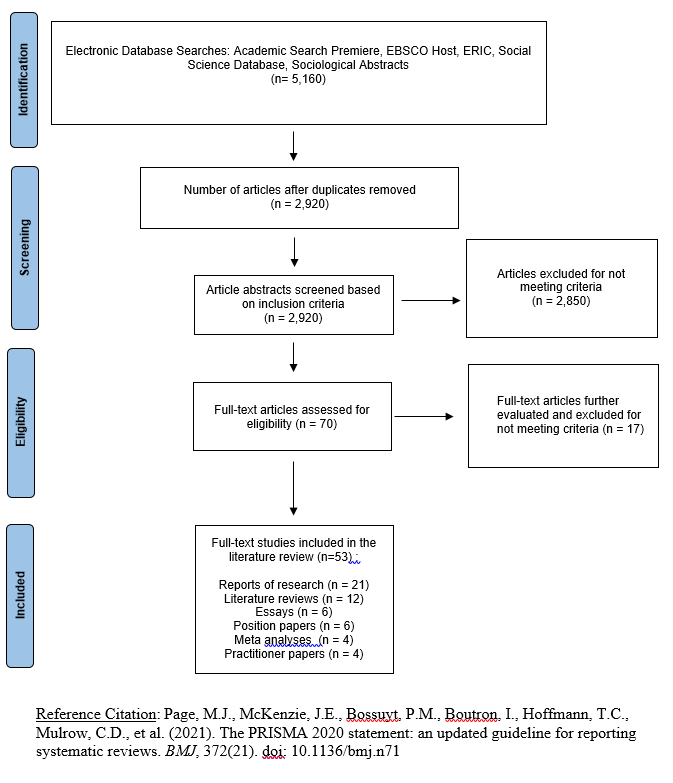
\includegraphics[width=8cm]{Figure 1.png}
 \caption{PRISMA Diagram for the Search of Research Literature and Selection of Articles }
    \label{PRISMA Diagram for the Search of Research Literature and Selection of Articles}
\end{figure}

\section*{PRISMA}
We utilized the PRISMA (Preferred Reporting Items for Systematic reviews and Meta- Analyses) method utilizing best-practices depicted with a flow diagram (see Figure 1) to “prepare a transparent, complete, and accurate account” (Page et al., 2021, p.1) of why we conducted this literature review, what we did, and what we found. The specific PRISMA process that was  followed in our review consisted of three steps in order: (1) Identification: Records were identified through database searching; (2) Screening: Records were screened for eligible, records sought for retrieval, and full-text articles assessed for eligibility; (3) Included: Total number of studies that were included in the review. Each step is separately detailed below.  

\section*{\textit{Identification}}
 
We started with a broad definition of STEM as referring to any one of the four fields – science, technology, engineering, and mathematics – as well as the integration of two or more fields (Honey et al., 2014). We conducted a search of electronic research databases, including EBSCO Host, Academic Search Premiere, ERIC, Social Science Database, and Sociological Abstracts, by applying combinations of ‘high school students with disabilities’ and the STEM terms. We enabled the search engine to use related words and terms. In this step, we applied these filters: peer-reviewed articles, in English, and published in the year 2000 or later. This process yielded a total of 5,160 articles. We then searched through this set of articles and deleted duplicates, which yielded a total of 2,920. The next step in the PRISMA process, screening, further reduced the total number of articles for this review based on the inclusion criteria.  

\section*{\textit{Screening}}

We downloaded articles from the databases and sorted them into two categories, relevant and not relevant. Relevant articles included any one of these criteria: (a) addressed high-school SWD preparing for or engagement in STEM careers, (b) high-school educator professional development for STEM, or (c) high school-level STEM program or curriculum. This process yielded 70 full-text articles deemed relevant by a consensus of all the authors. We independently read these articles applying the inclusion criteria. Then we met, and together we further scrutinized these articles. Based on the meeting and discussion, we excluded an additional 17 full-text articles and selected a final set of 53 full-text articles to review.

\section*{\textit{Included}}

These 53 selected articles are marked with an asterisk in the References section. The first and second authors took these articles and imported the PDF files into NVivo 12 (QSR, 2019), a software commonly used for qualitative data analyses. Because we utilized qualitative methodology for conducting this literature review, we followed best practices in qualitative research in education for ensuring trustworthiness and credibility, which included (a) reaching data saturation to include different perspectives and enhance richness of information, (b) triangulating different sources of data, (c) acknowledging how researcher perspectives, beliefs, and biases influence data collection and findings (i.e., reflexivity), (d) coding independently for initial review and then conducting consensus coding to develop final codes, and (e) minimizing reactivity through neutral stances and questions (Brantlinger et al., 2005).  

The first and second authors read and reviewed each article independently and applied start codes (Miles et al., 2014) on all 53 articles in the NVivo software. To ensure thorough and consistent coding, they defined the codes using examples and non-examples (Rossman \& Rallis, 1998) culled from the articles. Next, the authors extracted 'node reports’ from the NVivo software (a feature of the software) in order to inspect and identify main codes and sub-code extensions. The authors then selected 30 articles at random to conduct interrater agreement for coding using Cohen’s Kappa (Cohen, 1960), and produced a coefficient of .73. This value represented the proportion of coders’ agreement across the 30 articles taking into account coders’ chance agreement (McHugh, 2012). The authors completed consensus coding, and derived the themes to answer the two questions that framed this literature review.

\section*{Findings}

A summary of the 53 articles included this literature review is provided in Table 1; (see end of document) they are also indicated with an asterisk for the corresponding citation in the Reference section. These articles were published between 2000 and 2020 in 36 peer-reviewed journals, and a plurality (n=21) were research reports using qualitative, quantitative, or mixed methods. The remaining included articles were literature reviews (n=12), essays (n=6), position papers (n=6), meta-analysis (n=4), and practitioner papers (n=4). Our analyses of the 53 articles produced findings in the form of qualitative themes, which also constituted answers to the two questions and sub-questions (described earlier in the introduction) that framed this review. 

\section*{\textit{First Question: Preparing High-School SWD for STEM Careers}}
 
For the first review question, our analysis of selected literature resulted in four emergent themes: (a) barriers to STEM, (b) increasing STEM opportunities, (c) STEM readiness in college and career, and (d) STEM identity. Our analyses of the selected literature also produced sub-themes for two of these themes, barriers to STEM and increasing STEM opportunities.   

\section*{\textit{Theme 1: barriers to STEM}}

This theme emerged as the area of the relevant literature receiving the most research attention. Three specific types of barriers (i.e., sub-themes) were prominent: (a) lack of STEM experiences, (b) inaccessible classroom or school environments, and (c) lack of access to STEM curriculum. Examples of these sub-themes included traditional approaches to STEM that rely on substantial memorization (Scruggs et al., 2008; Villanueva \& Hand, 2011), complex and dense STEM content that places significant demands on working memory and attention (Basham et al., 2010; Boyle, 2012; Isaacson \& Michaels, 2015; Mason \& Hedin, 2011), limited STEM access due to negative stereotypes and expectations (Basham \& Marino, 2013; Dunn et al., 2012), and inadequate accommodations (Rule \& Stefanich, 2012). Barriers to STEM also involved the intersectionality of student disability with socioeconomic status (SES), gender, and race/ethnicity (Mau \& Li, 2018; Wang \& Degol, 2017), which presents implications for STEM education and career pathways, as diverse SWD become an increasingly larger share of the postsecondary education population and the workforce in STEM occupations (Byars-Winston, 2014).   

\section*{\textit{Theme 2: increasing STEM opportunities}}

For this theme, two specific opportunities for increasing STEM opportunities (i.e., sub-themes) were prominent: (a) expanding STEM programs by program and setting, and (b) recruiting and supporting SWD in STEM. Examples of these sub-themes included summer science camp for those with visual impairment (Supalo et al., 2011; Supalo et al., 2014); financial supports and off-campus internships in STEM (Leddy, 2010; Shoffner et al., 2015); STEM learning communities (Izzo et al., 2011; Peters-Burton et al., 2014) and use of different spaces at school for STEM learning (Subramaniam et al., 2012); supports and mentorships in STEM (Dunn et al., 2012), and increasing institutional commitment to recruiting, retaining, and graduating SWD into STEM fields (Marino \& Beecher, 2010).

\section*{\textit{Theme 3: STEM readiness in college and career }}

This theme appeared to be more sparse and emerging than the other areas (i.e., themes) of the relevant literature (above). Research suggests that high-school SWD need rigorous curriculum to prepare for STEM in career or college, but that alone is insufficient (Gottfried et al., 2016). They also need work-based experiences (Cease-Cook et al., 2015), which would involve partnerships with organizations in the community to provide those experiences, as well as career-technical education (CTE) (Sublett \& Plasman, 2017) or other applied STEM courses while in high school (Plasman \& Gottfried, 2018), and other STEM learning opportunities such as in-school field-trips and or out-of-school tutoring (Rakich \& Tran, 2016).  


\section*{\textit{Theme 4: STEM identity }}
  
This theme represents the newest area of the relevant literature. Thus, we found the fewest number of studies in our search. STEM identity and its often-associated area of social-emotional learning (SEL) have historically received the least research attention in special education, perhaps, due in part to construct and data complexity, with interconnected and contextualized variables such as identity, self-efficacy, and self-confidence. Gregg et al. (2017) studied the effects of virtual mentoring, using devices and platforms such as email, smartphones, and social media, on persistence in STEM for high-school SWD. The authors found that the largest improvements were in their perceptions of self-advocacy and self-determination, although these outcomes differed by student disability type and ethnicity. Likewise, analyzing nationally representative data of high school students, Sublett and Plasman (2017) reported that applied STEM coursework was predictive of self-efficacy increases in science and math for males without disabilities, but not for females or for SWD.    

\section*{\textit{Second Question: Preparing Educators to Support SWD in STEM}}

For the second review question, our analysis of selected literature resulted in three emergent themes: (a) individualizing learning and supports for SWD, (b) using technology and collaboration among educators, and (c) professional development. Our analyses of the literature did not produce any sub-themes for these three themes. 

\section*{\textit{Theme 1: individualizing learning and supports for SWD}}
 This theme was the most prominent among the themes relating to educators supporting high-school SWD in STEM. Project or inquiry-based learning and instruction are increasingly being recommended as significant elements of support for SWD (Kaldenberg et al., 2015; Seifert \& Espin, 2012; Therrien et al., 2011; Therrien et al., 2014). One example of this approach, the Science Writing Heuristic, involves designing learning templates for SWD and teachers (e.g., Villanueva \& Hand, 2011). Other approaches include the use of graphic organizers (Carnahan et al., 2016; Dexter et al., 2011). King et al. (2016) suggest that any of these approaches utilize, at a minimum, explicit instruction with prompts and positive reinforcement. 

Other researchers, such as Hwang and Taylor (2016) and Brigham et al. (2011), advocate individualizing of supports for SWD in STEM by (a) taking an interdisciplinary approach to supporting SWD in STEM, (b) collaborating across each STEM area, and (c) making direct connections to other disciplines, such as literature. An example of an interdisciplinary approach gaining favor among educators is called “STEAM” first developed at the Rhode Island School of Design. The argument is that incorporating the arts strengthens the curriculum for SWD by (a) motivating students especially when accessing the difficult aspects of STEM; (b) providing opportunities for self-expression, an important element in learning; and (c) serving as scaffolding for SWD to learn abstract and theoretical concepts in STEM. 

Other research suggests co-teaching model could be an effective way to support and accommodate SWD in general education STEM (Moorehead \& Grillo, 2013). Such a model would allow each teacher to focus on their respective strengths – the general educator as content knowledge specialist and the special educator as differentiation specialist. Mastropieri and Scruggs (2001), Mastropieri et al., (2005), and Scruggs et al. (2007) found that while teachers favorably viewed co-teaching, it also presented challenges relating to the classroom, students, and school administration: (1) Special educators too often served more of a subordinate function rather than a true “co-” teacher; and (2) Research based effective practices for supporting SWD, such as mnemonics, self-monitoring, peer mentoring, were often not being utilized.       

\section*{\textit{Theme 2: using technology and collaboration among educators}}
 
Technology has often been utilized by educators to enhance access to STEM fields for SWD (Williams et al., 2015). For example, computing and computational thinking have been used to tailor STEM instruction (Israel et al., 2013; Israel et al., 2015). Benefits of this approach include improvements in (a) collaborative problem solving, (b) attitude about computer science, (c) higher-order thinking skills, and (d) creation of applied, real-world contexts for teaching algorithmic problem solving. Universal design for learning (UDL) could also play a key role through multiple means of representation, expression and action, and student engagement. Isaacson and Michaels (2015) evaluated Math Speak, a system for speaking mathematical expressions in a non-ambiguous manner, for teaching math to SWD, was generally effective in communicating math and chemistry concepts to students with blindness and visual impairments. Marino and Beecher (2010) analyzed a Response-to-Intervention (RTI) approach incorporating video games to support STEM for students with learning disabilities. They found video games aided teachers in progress monitoring; video-game interface provided a way for teachers to collect assessment data in real time. Hart and Whalon (2012) analysis of self-management and technology strategies in science comprehension produced mixed results.

\section*{\textit{Theme 3: professional development }}

This theme represents an increasingly important area of the research literature. Yore and Treagust (2006) placed a greater focus and emphasis on teachers’ understanding the importance of students’ vocabulary acquisition in science learning and literacy. Along those lines, Taylor et al. (2020) recommended inquiry-based instruction for SWD in STEM be an integral part of teachers’ pre-service training and PD. This included explicit instruction in science vocabulary acquisition and retention, and the use of direct instruction, and mnemonics, as these elements have accumulated evidence in the research literature for their effectiveness in instructional supports for SWD. Kahn et al. (2017) reported that teacher candidates tended to primarily rely on SWD seeking help from other students before and after instruction, rather than being directly involved in designing environments and developing supports for SWD that would more likely foster student autonomy. In addition, there are other supplemental programs outside of the school environment that can offer PD opportunities in STEM for special education teachers, for example, the “Sci Train”, a project funded by the NSF designed to provide high-school science and math teachers effective methods of instruction, including the understanding and application of modifications and accommodations, and developing a resource library of these methods (Moon et al., 2012). Others have argued that the traditional classroom approach have ignored or hindered the essential element of innovative teaching, the ability of teachers to utilize their experiences, knowledge, and other unique personal factors to teach STEM (Fore et al., 2015).    

\section*{Discussion}
Our analyses of 53 selected articles from the relevant literature produced several themes and sub-themes to answer two specific questions. Now, we turn to a discussion of how those findings provide meaningful contributions to the literature, while also pointing to  knowledge gaps that remain. We then conclude this review with its limitations, and the implications in the field of education and special education for both research and practice.  

\section*{\textit{Qualitative Themes and Research Gaps}}
Significant changes have occurred in U.S. education related to STEM and high-school SWD, particularly since the passage of two landmark national laws, ‘No Child Left Behind’ in 2001 and ‘Individuals with Disabilities Education Improvement Act’ in 2004. Those changes are reflected in the peer-reviewed research; and thus, our present literature review was an attempt to capture the breadth and scope of that research over the last two decades. Taken together, the four themes that answered the first review question and the three themes that answered the second review question form an interesting – albeit preliminary – narrative regarding high-school SWD and STEM, and the role of educators, and leaving other questions to answer in the future. 

\section*{\textit{First review question and themes}}
The first review question was “How are high-school SWD prepared for careers in STEM?”, and our analyses of the selected literature yielded four emergent themes: (a) barriers to STEM, (b) increasing STEM opportunities, (c) STEM readiness in college and career, and (d) STEM identity. Based on our analyses, the focus of the literature appears to be on barriers and increasing opportunities in STEM for high-school SWD, but there are differences. For example, a female tenth-grade student of color with a learning  disability might experience some similar but also some different barriers in STEM than a male eleventh-grade student with autism. Also, increasing STEM opportunities through summer science-camp or active recruitment and retention into STEM programs, may be impactful for some but not others based on disability conditions. In reviewing a decade of NSF-funded research aimed at broadening participation of SWD in STEM, Thurston et al. (2017) found that barriers have become entrenched over decades. These include discrimination, lowered expectations, lack of access to facilities and adaptive technologies, and lack of resources and knowledge/skills by teachers. These barriers are connected to wider, systemic socioeconomic disparities (Falkenheim et al., 2017). For example, SWD are (a) less likely to graduate from college or university in a STEM major (National Science Foundation, 2019), (b) more likely to be unemployed or under-employed, and (c) more likely to live in poverty (Semega et al., 2019). Even adults with disabilities who have earned STEM degrees have experienced (a) fewer opportunities in internships and research assistantships, (b) less funding from scholarships and grants, and (c) higher unemployment rates in STEM fields than their peers without disabilities (National Science Foundation, 2021). 

While the problem of barriers in STEM for SWD and the interventions to address them (e.g., project-based learning and universal design) (e.g., Bargerhuff, 2013) have been well-studied (see Scruggs \& Mastropieri, 2007), there remain gaps in knowledge. For example, there is still not a good understanding of how these approaches and others, such as summer STEM programs, produce large scale (i.e., across different student-disability groups and settings) or long-term positive effects (i.e., from grade school through post-high school). Part of this gap could be due, at least in part, to the complex multilevel interactions of many variables (e.g., Austin \& Merlo, 2017) involved in STEM success for SWD, including but not limited to disability, demographics, family dynamics, school and district factors, and the contextualized nature of how IEPs are developed and implemented by educators for SWD. 

In addition, while STEM identity for high-school SWD is an important emerging area of research, there is still very little understanding of how it develops in the early years of schooling, from primary to middle grades (see Wang \& Degol, 2017) affecting the trajectory in later years. Moreover, while there is increased understanding of the connection between STEM identity and social-emotional learning for students in general education, this research is lacking in special education. Finally, there is very little empirical understanding of the developmental pathways through which STEM identity of SWD translates to STEM success, and how this process differs among their peers without disabilities, from high-school to college, or from high school to STEM workforce in traditional and ‘hidden’ STEM fields (see Rothwell, 2013).  
    

\section*{\textit{Second review question and themes}}
The second review question was, “How are educators prepared to support high school SWD for opportunities in STEM?”; and our analyses produced three emergent themes: (a) individualizing learning and supports for SWD, (b) using technology and collaboration among  educators, and (c) professional development. Based on our analyses, the focus of the literature in this specific area of research appears to be individualizing the learning experience and supports for high-school SWD in STEM, and utilizing more regular professional development of educators to keep up with the changes in STEM areas (e.g., new technologies, new scientific applications). The narrative focuses on educators and their pivotal role in the high-school STEM success for SWD, and in their post-high school transition to STEM career pathways.

What stood out in particular in this area of the literature was the emphasis, at a classroom level, of the utilization of project based or inquiry based learning, coupled with the emphasis on direct instruction (see Rizzo \& Taylor, 2016). Much of this research focus is weighed toward reading (i.e., vocabulary, comprehension) STEM texts for high-school students with a specific learning disability (SLD) and autism spectrum disorder (ASD). Some of this focus can be explained by the fact that the largest group of SWD served in special education in the U.S. are those with SLD, and the fastest growing group of SWD are those with ASD (National Center for Education Statistics, 2022). What is still a significant gap in this research, however, is that there are 11 other categories of disabilities under IDEA for which SWD can be served in special education. Clearly much more research is needed regarding high-school students with these other disabilities, about how well (or different) project/inquiry-based learning and direct instruction affect their STEM learning and outcomes, and whether those approaches differ in effectiveness across the STEM areas – science, technology, engineering, and mathematics.  

The literature also pointed to a more emerging area of research, involving specialized, STEM-specific professional development of educators. This could include active collaboration of teachers in general education and special education in both STEM instruction and supports for high-school SWD (see Moon et al., 2012). Perhaps this push for collaboration reflects the sheer complexity of STEM instruction and supporting high-school SWD, something that requires more than what special educators can reasonably endeavor all on their own. For example, content knowledge in the four STEM areas – science, technology, engineering, and mathematics – also covers subject matter that includes biology, chemistry, geology, physics, astronomy, computer science, and material science. The issue here, however, is that given the resources challenges that many schools and districts have across the country, specialized professional development for both general educators (e.g., direct instruction to support high-school SWD learning in STEM) and special educators (e.g., computer programming in Java) may be difficult or very limited. 

\section*{\textit{Limitations of This Qualitative Review}}
There were three main limitations in this literature review. First, although we used search terms in various combinations and searched multiple databases, it is still possible that our search was too narrow. Second, while we followed an inclusion criteria driven by specific questions, it is likely that additional and or different patterns could be identified by others who reviewed the same literature. Third, the studies that were research reports varied in rigor; only a few of these are likely to meet the strict “What Works Clearinghouse” criteria  (https://ies.ed.gov /ncee/wwc/)  for establishing evidence-based practices in education. This puts a limitation on how educators could use information from this review – or the individual results of each of those research reports directly – in whatever program, practice, or policy at their school or in their district.  

Finally, we acknowledge that the inclusion of different types of articles in our literature review reflects not only the diversity of thoughts and writings in the field, but also the challenges of conducting research specific to STEM and high-school SWD. While very few of these studies have been assessed as having sufficient methodological rigor to meet the standards of the “What Works Clearinghouse”, the inclusion of these ‘other’ types of articles – essays, literature reviews, meta-analyses, position papers, and practitioner papers – and the development of qualitative themes across these articles were meant to portray or represent the current state (i.e., focus areas, emerging areas) of the peer-reviewed literature regarding high-school SWD and STEM.     

\section*{Implications for Research and Practice}
\section*{\textit{Implications for practice    }}
Research from the past twenty years has indicated that high-school SWD can achieve in STEM. Nevertheless, there remain disparities between students with and without disabilities as well as gaps in research knowledge. One clear implication of our review for educators, in both general and special education, is that the utilization of technology and active collaboration in STEM instruction are positive ways to support STEM learning for high-school SWD and increasing opportunities for both in-school and out-of-school learning. Because education in the U.S. is decentralized, individual schools and districts would need to take the initiative to create these opportunities, in addition to any federal programs or resource that could be utilized.  

Another implication of this review is that greater focus and attention needs to be given to the IEP process and transition planning for SWD starting at age 14, to identify and incorporate STEM activities into their high-school learning experiences to adequately prepare for college and or STEM career pathways. There is also a need for specialized STEM focused pre-service training and in-service professional development. Because STEM continues to evolve and technology continues to advance, these special educators will need to stay up-to-date in their knowledge, including the emerging research around STEM identity development for SWD.   

\section*{\textit{Implications for research}}
Despite the limitations of this qualitative literature review, there are important implications for research. Our review has revealed that there is room for much further investigation in a few key areas. One area is research into STEM enrichment programs (e.g., “Camp Can Do’), which provide out-of-school seasonal or periodic STEM learning opportunities for SWD based on disability category, gender, and race/ethnicity. This type of intersectionality research will also show the complexity of STEM learning, which manifests in different growth trajectories for high-school SWD based on these demographic characteristics (Wei et al., 2012). Second area of research is STEM identity and social-emotional learning, and how they influence SWD readiness to pursue STEM career pathways. These longitudinal studies will be key to understanding how SWD develop the necessary resilience and persistence over time, from high school and into college/university, and career in STEM. The third area involves STEM-focused high-school transition services in special education and their link to post-high school outcomes of SWD (i.e., IDEA requirement Indicator 14). This is an important area of special education that is becoming a greater focus of administrators and policymakers. Because high-school SWD are legally entitled to these services, conducting research to more closely analyze how IEP (Individualized Education Program) are structured for high-school SWD to prepare for post-high school STEM (i.e., college, career) could lead to developing best practices in transition services. 

\section*{\textit{Conflict of Interest Statement}}
The authors declare there is no conflict of interest.

\section*{\textit{Declaration of Funding}}
This study is part of research funded by the National Science Foundation grant #1657015.

\section*{\textit{Ethics statement}}
This paper was a review of extant literature and not a study involving human or animal subjects in research.

\include{} 
\section*{References}\par 

\leftskip 0.25in
\parindent -0.25in 
%%%

*Indicates studies reviewed in this paper 

Austin, P.C., \& Merlo, J. (2017). Intermediate and advanced topics in multilevel logistic regression analysis. \textit{Statistics in Medicine, 36}, 3257–3277. doi:10.1002/sim.7336

*Bargerhuff, M.E. (2013). Meeting the needs of students with disabilities in a stem school. \textit{American Secondary Education, 41}(3), 3-20. \url{https://doi.org/10.1002/tea.21437}

*Basham, J.D., \& Marino, M.T. (2013). Understanding STEM education and supporting students through universal design for learning. \textit{Teaching Exceptional Children, 45}(4), 8-15. \url{https://doi.org/10.1177%2F004005991304500401}

*Basham, J.D., Israel, M., \& Maynard, K. (2010). An ecological model of STEM education: Operationalizing STEM for all.\textit{ Journal of Special Education Technology, 25}(3), 9-19. \url{https://doi.org/10.1177%2F016264341002500303}

*Boyle, J.R. (2012). Note-taking and secondary students with learning disabilities: Challenges and solutions.\textit{ Learning Disabilities Research \& Practice, 27}(2), 90-101. \url{https://doi.org/10. 1177/0731948711435794}

Brantlinger, E., Jimenez, R., Klingner, J., Pugach, M., \& Richardson, V. (2005). Qualitative studies in special education. \textit{Exceptional Children, 71}(2), 195-207.

*Brigham, F.J., Scruggs, T.E., \& Mastropieri, M.A. (2011). Science education and students with learning disabilities. \textit{Learning Disabilities Research \& Practice, 26}(4), 223-232. \url{https://psycnet.apa.org/doi/10.1111/ j.1540-5826.2011.00343.x}

Bureau of Labor Statistics (2017). \textit{STEM Occupations: Past, Present, and Future} (Spotlight on Statistics by Stella Fayer, Alan Lacey, \& Audrey Watson). Retrieved from \url{https:// www.bls.gov/spotlight/2017/science- technology-engineering-and-mathematics-stem-occupations-past-present-and-future/home.htm}

Bureau of Labor Statistics (2020).\textit{ Employment projections: Employment in STEM occupations.} \url{https://www.bls.gov/emp/tables/stem-employment.htm}

*Byars-Winston, A. (2014). Toward a framework for multicultural STEM-focused career 
interventions. \textit{The Career Development Quarterly, 62}(4), 340-357. \url{https://doi.org/10.1002/ j.2161-0045.2014.00087.x}

*Carnahan, C.R., Williamson, P., Birri, N., Swoboda, C., \& Snyder, K.K. (2016). Increasing comprehension of expository science text for students with autism spectrum disorder. \textit{Focus on Autism and Other Developmental Disabilities, 31}(3), 208-220. \url{https://doi.org/ 10.1177/1088357615610539}

*Cease-Cook, J., Fowler, C., \& Test, D.W. (2015). Strategies for creating work-based learning experience in schools for secondary students with disabilities.\textit{ Teaching Exceptional Children, 47}(6), 352-358. \url{https://doi.org/10.1177/004005991558003}

Christenson, J. (2011). Ramaley coined STEM term now used nationwide. \textit{Winona Daily News}, 
November 13, 2011. \url{https://www. winonadailynews.com/news/local/ramaley-coined-stem-term-now-used-nationwide/article_457afe3e-0db3-11e1-abe0-001cc4c03286.html}

Chute, E. (2009). STEM education is branching out. \textit{Pittsburgh Post-Gazette}, February 10, 2009. \url{https://www.post-gazette.com/news/education/2009/02/10/STEM-education-is-branching-out/stories/200902100165}

Cohen, J. (1960). A coefficient of agreement for nominal scales. \textit{Educational and Psychological Measurement}, 20, 37–46.

*Dexter, D.D., Park, Y.J., \& Hughes, C.A. (2011). A meta-analytic review of graphic organizers and science instruction for adolescents with learning disabilities: Implications for the intermediate and secondary science classroom.\textit{ Learning Disabilities Research, 26}(4), 204-213. \url{https://doi.org/10.1111/j.1540-5826.2011.00341.x}

*Dunn, C., Rabren, K.S., Taylor, S.L., \& Dotson, C.K. (2012). Assisting students with high-incidence disabilities to pursue careers in science, technology, engineering, and mathematics. \textit{Intervention in School and Clinic, 48}(1), 47-54. \url{https://doi.org/10.1177/1053451212443151}

*Falkenheim, J., Burke, A., Muhlberger, P., \& Hale, K. (2017). \textit{Women, Minorities, and Persons with Disabilities in Science and Engineering: 2017}. National Science Foundation, National Center for Science and Engineering Statistics. 2017. Special Report NSF 17-310. Arlington, VA. \url{https://www.nsf.gov/statistics/wmpd/}

*Fore, G.A., Feldhaus, C.R., Sorge, B.H., Agarwal, M., \& Varahramyan, K. (2015). Learning at the nano-level: Accounting for complexity in the internalization of secondary STEM teacher professional development. \\\textit{Teaching and Teacher Education}, 51, 101-112. \url{http://dx.doi.org/10.1016/j.tate.2015.06.008}

Gerlach, J. (2012). \textit{STEM: Defying a simple definition}. National Science Teachers Association (NSTA) Web Digest. NSTA Reports April 11, 2012.

*Gottfried, M.A., Bozick, R., Rose, E., \& Moore, R. (2016). Does career and technical education strengthen the STEM pipeline? Comparing students with and without disabilities. \textit{Journal of Disability Policy Studies, 26}(4), 232-244. \url{https://doi.org/10.1177/1044207314544369}

*Gregg, N., Galyardt, A., Wolfe, G., Moon, N., \& Todd, R. (2017). Virtual mentoring and 
persistence in STEM for students with disabilities.\textit{ Career Development and Transition for Exceptional Children, 40}(4), 205-214. \url{http://doi.org/10.1177/2165143416651717}

*Hart, J.E., \& Whalon, K.J. (2012). Using video self-modeling via iPads to increase academic 
responding of an adolescent with autism spectrum disorder and intellectual disability. 
\textit{Education and Training in Autism and Developmental Disabilities, 47}(4), 438–446. \url{https://www.learntechlib.org/p/50203/}

Holmlund, T.D., Lesseig, K., \& Slavit, D. (2018). Making sense of “STEM education” in K-12 contexts. \textit{International Journal of STEM Education, 5}(32), 1-18. \url{https://doi.org/10.1186/s40594-018-0127-2}

Honey, M., Pearson, G., \& Schweingruber, H. (2014). \textit{STEM integration in K-12 education: status, prospects, and an agenda for research}. National Academy of Engineering and National Research Council. The National Academies Press: Washington, DC. \url{https://doi.org/10.17226/18612}

*Hwang, J., \& Taylor, J.C. (2016). Stemming on STEM: A STEM education framework for students with disabilities. \textit{Journal of Science Education, 19}(1), 39-49. \url{https://doi.org/10.14448/jsesd.09.0003}

Individuals with Disabilities Education Act, P.L. 108-446, codified as amended at title U.S.C. §20 U.S.C. 1400(d).

*Isaacson, M.D., \& Michaels, M. (2015). Ambiguity in speaking chemistry and other STEM content: Educational implications. \textit{Journal of Science Education for Students With Disabilities, 18}(1), 1-9. \url{https://doi.org/10.14448/jced.07.0001}

*Israel, M., Maynard, K., \& Williamson, P. (2013). Promoting literacy – Embedded, authentic STEM instruction for students with disabilities and other struggling learners.\textit{ Teaching Exceptional Children, 45}(4), 18-25. \url{https://doi.org/10.1177/004005991304500402}

*Israel, M., Wherfel, Q.M., Pearson, J., Shehab, S., \& Tapia, T. (2015). Empowering K-12 students with disabilities to learn computational thinking and computer programming. \textit{Teaching Exceptional Children, 48}(1), 45-53. \url{https://doi.org/10.1177/004005991559479}

*Izzo, M.V., Murray, A., Priest, S., \& McArrell, B. (2011). Using student learning communities to recruit STEM students with disabilities. \textit{Journal of Postsecondary Education and Disability, 24}(4), 301-316. \url{https://files. eric.ed.gov/fulltext/EJ966131.pdf}

*Kaldenberg, E.R., Watt, S.J., \& Therrien, W.J. (2015). Reading instruction in science for students with learning disabilities: A meta-analysis.\textit{ Learning Disability Quarterly, 38}(3), 160-173, \url{https://doi.org/10.1177/073194871 4550204}

*Kahn, S., Pigman, R., \& Ottley, J. (2017). A tale of two courses: Exploring teacher candidates’ translation of science and special education methods instruction into inclusive science practices. \textit{Journal of Science Education for Students with Disabilities, 20}(1), Article 6, 50-68. \url{http://scholarworks.rit.edu/ jsesd/vol20/iss1/6}

*King, S.A., Lemons, C.J., \& Davidson, K.A. (2016). Math interventions for students with autism spectrum disorder: A best-evidence synthesis. Exceptional Children, 82(4), 443-462. \url{https://doi.org/10.1177%2F0014402915625066}

*Leddy, M.H. (2010). Technology to advance high school and undergraduate students with disabilities in science, technology, engineering, and mathematics. \textit{Journal of Special Education Technology, 25}(3), 3-8. \url{https://www.learn techlib.org/p/113978/}

*Marino, M.T., \& Beecher, C.C. (2010). Conceptualizing RTI in 21st-century secondary science 
classrooms: Video games’ potential to provide tiered support and progress monitoring for students with learning disabilities.\textit{ Learning Disability Quarterly}, 33, 299-311. \url{https://doi.org/10.1177%2F073194871003300407}

*Mason, L.H., \& Hedin, L.R. (2011). Reading science text: Challenges for students with learning disabilities and considerations for teachers. \textit{Learning Disabilities: Research \& Practice}, 26, 214–222. \url{https://doi.org/10. 1111/j.1540-5826.2011.00342.x}

*Mastropieri, M., \& Scruggs, T.E. (2001). Promoting inclusion in secondary classrooms. \textit{Learning Disability Quarterly, 24}(4), 265-274. \url{https://doi.org?10.2307/1511115}

*Mastropieri, M.A., Scruggs, T.E. \& Graetz, J. (2005). “Cognition and learning in inclusive high 
school chemistry classes”. In\textit{ Advances in learning and behavioral disabilities: Vol. 18. 
Cognition and learning in diverse settings}, Edited by: Scruggs, T. E. and Mastropieri, M. 
A. 107–118. Oxford, United Kingdom: Elsevier.

*Mau, W-C. J., \& Li, J. (2018). Factors influencing STEM career aspirations of underrepresented high school students.\textit{ The Career Development Quarterly, 66}(3), 246-258. \url{https://doi.org/10.1002/cd.150}

McComas W.F. (2014) STEM: Science, Technology, Engineering, and Mathematics. In McComas W.F. (eds.). \textit{The Language of Science Education}. SensePublishers, Rotterdam. \url{https://doi.org/10.1007/978-94-6209-497-0_92}

McHugh, M.L. (2012). Interrater reliability: The Kappa statistic. \textit{Biochemia Medica, 22}(3), 276-282. \url{https://doi.org:10.11613/ BM.2012.031}

Miles, M.B., Huberman, A.M., \& Saldaña, J. (2014).\textit{ Qualitative data analysis: A methods sourcebook} (3rd ed). Los Angeles, CA: Sage Publications. 

*Moon, N.W., Todd, R.L., Morton, D.L., \& Ivey, E. (2012). \textit{Accommodating students with disabilities in science, technology, engineering, and mathematics (STEM): Findings from research and practice for middle grades through university education}. A publication of SciTrain: Science and Math for All, sponsored by the National Science Foundation (Award No. 0622885). Atlanta, GA: Center for Assistive Technology and Environmental Access, College of Architecture, Georgia Institute of Technology. \url{https://hourofcode.com/files/accommodating-students-with-disabilities.pdf}

*Moorehead, T., \& Grillo, K. (2013). Celebrating the reality of inclusive STEM education: Co-teaching in science and mathematics. \textit{Teaching Exceptional Children, 54}(4), 50-57. \url{https://journals.sagepub.com/doi/pdf/10.1177/004005991304500406}

National Center for Education Statistics. (2015).\textit{ National assessment of educational progress 4th grade science assessment}. Washington, D.C.: Institute of Education Sciences.

National Center for Education Statistics. (2022).\textit{ Students with Disabilities: Percentage distribution of students ages 3–21 served under the Individuals with Disabilities Education Act (IDEA), by disability type: School year 2020–21}.

National Science Foundation (2019).\textit{ Women, minorities, and persons with disabilities in science and engineering}. National Center for Science and Engineering Statistics, Directorate for Social, Behavioral and Economic Sciences. \url{https://ncses.nsf.gov/pubs/nsf19304/digest}

National Science Foundation (2021).\textit{ Women, minorities, and persons with Disabilities in science and engineering}. National Center for Science and Engineering Statistics. Special Report NSF 21-321. Alexandria, VA. \url{https://ncses.nsf.gov/wmpd}

Onwuegbuzie, A.J., Leech, N.L., \& Collins, K.M.T. (2012). Qualitative analysis techniques for the review of the literature.\textit{ Qualitative Report, 17}(56), 1-28. \url{http://www.nova.edu/\\ssss/QR/QR17/onwuegbuzie.pdf}

Page, M.J., McKenzie, J.E., Bossuyt, P.M., \\Boutron, I., Hoffmann, T.C., Mulrow, C.D., et al. (2021). The PRISMA 2020 statement: an updated guideline for reporting systematic reviews. \textit{BMJ}, 372(21). doi: 10.1136/bmj.n71

Paré G., Trudel, M.C., Jaana, M., \& Kitsiou, S. (2015) Synthesizing information systems knowledge: A typology of literature reviews.\textit{ Information \& Management. 52}(2), 183-199. \url{http://dx.doi.org/10.1016/j.im.2014.08.008}

*Peters-Burton, E.E., Lynch, S.J., Behrend, T.S., \& Means, B.B. (2014). Inclusive STEM high school design: 10 critical components. \textit{Theory Into Practice}, 53, 64-71. \url{https://doi.org/\\10.1080/00405841.2014.862125}

*Plasman, J.S., \& Gottfried, M.A. (2018). Applied STEM coursework, high school dropout rates, and students with learning disabilities. \textit{Educational Policy}, 32(5), 664-696. \url{https://doi.org/10.1177/0895904816673738}

QSR (2019). \textit{NVivo Qualitative Data Analysis Software }(Version 12) [Computer Software]. Burlington, MA: QSR International (Americas) Inc.

*Rakich, S.S., \& Tran, V. (2016) A Balanced Approach to Building STEM College and Career Readiness in High School: Combining STEM Intervention and Enrichment Programs. \textit{European Journal of STEM Education, 1}(3), p.59. \url{http://dx.doi.org/10.20897/lectito.201659}

*Rizzo, K.L., \& Taylor, J.C. (2016). Effects of inquiry-based instruction on science achievement for students with disabilities: An analysis of the literature.\textit{ Journal of Science Education for Students with Disabilities, 19}(1), Article 2, 1-16. \url{https://scholarworks.rit.edu/\\jsesd/vol19/iss1/2/}

Rossman, G.B., \& Rallis, S.F. (1998). \textit{Learning in the Field: An introduction to qualitative 
research}. Thousand Oaks, CA: Sage Publications, Inc.

Rothwell, J. (2013). \textit{The hidden STEM economy: The metropolitan policy program at Brookings}. Washington, DC: Brookings Institution. \url{https://www.brookings.edu/research/the-hidden-stem-economy}

*Rule, A.C., \& Stefanich, G.P. (2012). Using a thinking skills system to guide discussions during a working conference on students with disabilities pursuing STEM fields. \textit{Journal of STEM Education}, 13(1), 43-54. \url{https://gseuphsdlibrary.files.wordpress.com/2013/03/using-a-thinking-skills-system-to-guide-discussions-during-a-working-conference-on-students-with-disabilities-pursuing-stem-fields.pdf}

Sanders, M. (2009). STEM, STEM education, STEMmania. \textit{The Technology Teacher}, 68(4),
20-26.

*Scruggs, T.E., \& Mastropieri, M.A. (2007). Science learning in special education: The case for 
constructed versus instructed learning. \textit{Exceptionality}, 15, 57-74. \url{https://doi.org/\\10.1080/09362830701294144}

*Scruggs, T.E., Mastropieri, M.A., \& McDuffie, K.A. (2007). Co-teaching in inclusive classrooms: A meta-synthesis of qualitative research. \textit{Exceptional Children}, 73(4),
392-416. \url{https://doi.org/10.1177%2F001440290707300401}

*Scruggs, T.E., Mastropieri, M.A., \& Okolo, C.M. (2008). Science and social studies for students with disabilities. \textit{Focus on Exceptional Children}, 41(2), 1-24.

*Seifert, K., \& Espin, C. (2012). Improving reading of science text for secondary students with learning disabilities: Effects of text reading, vocabulary learning, and combined approaches to instruction. \textit{Learning Disability Quarterly}, 35(4), 236-247. \url{https://doi.org/10.1177/0731948712444275}

Semega, J., Kollar, M., Creamer, J., \& Mohanty, A. (2019).\textit{ Income and poverty in the United 
States: 2018 }(Current Population Reports P60-266). Washington, D.C.: U.S. Census Bureau (U.S. Government Printing Office). \url{https://www.census.gov/content/dam/Census/library/publications/2019/demo/p60-266.pdf}

*Shoffner, M.F., Newsome, D., Minton, C.A., \& Morris, C.A. (2015). A qualitative exploration of the STEM career-related outcome expectations of young adolescents. \textit{Journal of Career Development}, 42(2), 102-116. \url{https://doi.org/10.1177/0894845314544033}

Snyder, H. (2019). Literature review as a research methodology: An overview and guidelines. \textit{Journal of Business Research}, 104, 333-339.

*Sublett, C., \& Plasman, J.S. (2017). How does applied STEM coursework relate to mathematics  and science self-efficacy among high school students? Evidence from a national sample. \textit{Journal of Career and Technical Education}, 32(1), 29-50. \url{http://doi.org/10.21061/jcte.v32i1.1589}

*Subramaniam, M.M., Ahn, J., Fleischmann, K.R., \& Druin, A. (2012). Reimagining the role of school libraries in STEM education: Creating hybrid spaces for exploration. \textit{The Library Quarterly: Information, Community, Policy}, 82(2), 161-182. \url{https://doi.org/10.1086/664578}

*Supalo, C.A., Isaacson, M.D., \& Lombardi, M.V. (2014). Making hands-on science learning for students who are blind or have low vision. \textit{Journal of Chemical Education}, 91, 195-199. \url{https://doi.org/10.1021/ed3000765}

*Supalo, C.A., Wohlers, H.D., \& Humphrey, J.R. (2011). Students with blindness explore 
chemistry at ‘Camp Can Do’.\textit{ Journal of Science Education for Students with Disabilities}, 15(1), 1-9. \url{https://doi.org/:10.14448/jsesd.04.0001}

*Taylor, J.C., Rizzo, K.I., Hwang, J., \& Hill, D. (2020). A review of research on science instruction for students with autism spectrum disorder.\textit{ School Science and Mathematics}, 120, 116-125. \url{https://doi.org/10.1111/ssm.1238}

*Therrien, W.J., Taylor, J.C., Hosp, J.L., Kaldenberg, E.R., \& Gorsh, J. (2011). Science instruction for students with learning disabilities: A meta-analysis. \textit{Learning Disabilities Research \& Practice}, 26(4), 188-203. \url{https://doi.org/10.1111/j.1540-5826.2011.00340.x}

*Therrien, W.J., Taylor, J.C., Watt, S., \& Kaldenberg, E. (2014). Science instruction for students with emotional and behavioral disorders.\textit{ Remedial and Special Education}, 35(1), 15-27. \url{https://doi.org/10.1177/07419 32513 503557}

Thurston, L.P., Shuman, C., Middendorf, B.J., \& Johnson, C. (2017). Postsecondary STEM education for students with disabilities: Lessons learned from a decade of NSF funding. \textit{Journal of Postsecondary Education and Disability}, 30(1), 49-60. \url{https://files.eric.ed.gov/\\fulltext/EJ1144615.pdf}

*Villanueva, M.G., \& Hand, B. (2011). Science for all: Engaging students with special needs in and about science. \textit{Learning Disabilities Research \& Practice}, 26(4), 233–240. \url{https://\\doi.org/10.1111/j.1540-5826.2011.00344.x}

*Wang, M-T., \& Degol, J.L. (2017). Gender gap in science, technology, engineering, and mathematics (STEM): Current knowledge, implications for practice, policy, and future directions. \textit{Educational Psychology Review}, 29(1), 119-140. \url{https://doi.org/10.1007/s10648-015-9355-x}

*Wei, X., Lenz, K. B., \& Blackorby, J. (2012). Math growth trajectories of students with disabilities: Disability category, gender, racial, and socioeconomic status differences from ages 7 to 17. \textit{Remedial and Special Education}, 34(3), 154-165. \url{https://doi.org/10.1177/0741932512 448253}

*Williams Jr., T.O., Ernst, J.V., \& Kaui, T.M. (2015). Special populations at-risk for dropping out of school: A discipline-based analysis of STEM educators. \textit{Journal of STEM Education}, 16(1), 41-45. \url{https://vtechworks.lib.vt.edu/bitstream/handle/10919/76635/WilliamsSpecialPopulations2015.pdf?sequence=1\&isAllowed=y}

*Yore, L.D., \&Treagust, D.F. (2006). Current realities and future possibilities: Language and science literacy—empowering research and informing instruction.\textit{ International Journal of Science Education}, 28(2-3), 291-314. \url{https://doi.org/10.1080/09500690500336973}
\pagebreak

\include{} 


\endleftskipleftskip 
\endparindentparindentparindentparindent

\newpage
\pagebreak

\clearpage

% Please add the following required packages to your document preamble:
% \usepackage{graphicx}
\begin{table*}[]
\caption{Summary of Articles (N=53) Selected for the Qualitative Literature Review}
\label{tab:my-table}
\resizebox{\textwidth}{!}{%
\begin{tabular}{llllllll}
\hline
\multicolumn{1}{c}{\textbf{Authors}} &
  \multicolumn{1}{c}{\textbf{Journal}} &
  \multicolumn{1}{c}{\textbf{Design}} &
  \multicolumn{1}{c}{\textbf{Sample}} &
  \multicolumn{1}{c}{\textbf{Disability}} &
  \multicolumn{1}{c}{\textbf{Ethnicity}} &
  \multicolumn{1}{c}{\textbf{Gender}} &
  \multicolumn{1}{c}{\textbf{Topics}} \\ \hline
\begin{tabular}[c]{@{}l@{}}Bargerhuff \\ (2013)\end{tabular} &
  \begin{tabular}[c]{@{}l@{}}American \\ Secondary \\ Education\end{tabular} &
  Qualitative &
  \begin{tabular}[c]{@{}l@{}}education \\ professionals \\ (N=9)\end{tabular} &
  \begin{tabular}[c]{@{}l@{}}Not \\ Available\end{tabular} &
  \begin{tabular}[c]{@{}l@{}}Not \\ Available\end{tabular} &
  \begin{tabular}[c]{@{}l@{}}females \\ (n=7), \\ males \\ (n=2)\end{tabular} &
  \begin{tabular}[c]{@{}l@{}}Project-\\ based STEM \\ learning, \\ problem-\\ solving\end{tabular} \\ \hline
\begin{tabular}[c]{@{}l@{}}Basham \& \\ Marino \\ (2013)\end{tabular} &
  \begin{tabular}[c]{@{}l@{}}Teaching \\ Exceptional \\ Children\end{tabular} &
  \begin{tabular}[c]{@{}l@{}}Position \\ paper\end{tabular} &
  \begin{tabular}[c]{@{}l@{}}Not \\ Applicable\end{tabular} &
  \begin{tabular}[c]{@{}l@{}}Not \\ Applicable\end{tabular} &
  \begin{tabular}[c]{@{}l@{}}Not \\ Applicable\end{tabular} &
  \begin{tabular}[c]{@{}l@{}}Not \\ Applicable\end{tabular} &
  \begin{tabular}[c]{@{}l@{}}UDL in \\ STEM \\ instruction\end{tabular} \\ \hline
\begin{tabular}[c]{@{}l@{}}Basham, Israel, \\ \& Maynard \\ (2010)\end{tabular} &
  \begin{tabular}[c]{@{}l@{}}Journal of \\ Special \\ Education \\ Technology\end{tabular} &
  Essay &
  \begin{tabular}[c]{@{}l@{}}Not \\ Applicable\end{tabular} &
  \begin{tabular}[c]{@{}l@{}}Not \\ Applicable\end{tabular} &
  \begin{tabular}[c]{@{}l@{}}Not \\ Applicable\end{tabular} &
  \begin{tabular}[c]{@{}l@{}}Not \\ Applicable\end{tabular} &
  \begin{tabular}[c]{@{}l@{}}Framework \\ for more \\ accessible \& \\ effective \\ STEM \\ instruction\end{tabular} \\ \hline
\begin{tabular}[c]{@{}l@{}}Boyle \\ (2012)\end{tabular} &
  \begin{tabular}[c]{@{}l@{}}Learning \\ Disabilities \\ Research \\ \& Practice\end{tabular} &
  \begin{tabular}[c]{@{}l@{}}Literature \\ review\end{tabular} &
  \begin{tabular}[c]{@{}l@{}}Not \\ Applicable\end{tabular} &
  \begin{tabular}[c]{@{}l@{}}Learning \\ Disability\end{tabular} &
  \begin{tabular}[c]{@{}l@{}}Not \\ Applicable\end{tabular} &
  \begin{tabular}[c]{@{}l@{}}Not \\ Applicable\end{tabular} &
  \begin{tabular}[c]{@{}l@{}}High school \\ content \\ areas, note-\\ taking\end{tabular} \\ \hline
\begin{tabular}[c]{@{}l@{}}Brigham, \\ Scruggs, \& \\ Mastropieri \\ (2011)\end{tabular} &
  \begin{tabular}[c]{@{}l@{}}Learning \\ Disabilities \\ Research \\ \& Practice\end{tabular} &
  \begin{tabular}[c]{@{}l@{}}Literature \\ review\end{tabular} &
  \begin{tabular}[c]{@{}l@{}}Not \\ Applicable\end{tabular} &
  \begin{tabular}[c]{@{}l@{}}Learning \\ Disability\end{tabular} &
  \begin{tabular}[c]{@{}l@{}}Not \\ Applicable\end{tabular} &
  \begin{tabular}[c]{@{}l@{}}Not \\ Applicable\end{tabular} &
  \begin{tabular}[c]{@{}l@{}}Validated \\ science \\ teaching \\ strategies\end{tabular} \\ \hline
\begin{tabular}[c]{@{}l@{}}Byars-Winston \\ (2014)\end{tabular} &
  \begin{tabular}[c]{@{}l@{}}The Career \\ Development \\ Quarterly\end{tabular} &
  Essay &
  \begin{tabular}[c]{@{}l@{}}Not \\ Applicable\end{tabular} &
  \begin{tabular}[c]{@{}l@{}}Not \\ Applicable\end{tabular} &
  \begin{tabular}[c]{@{}l@{}}Not \\ Applicable\end{tabular} &
  \begin{tabular}[c]{@{}l@{}}Not \\ Applicable\end{tabular} &
  \begin{tabular}[c]{@{}l@{}}STEM \& \\ career, \\ under-\\ represented \\ groups\end{tabular} \\ \hline
\begin{tabular}[c]{@{}l@{}}Carnahan, \\ Williamson, \\ Birri, Swoboda, \\ \& Snyder \\ (2016)\end{tabular} &
  \begin{tabular}[c]{@{}l@{}}Focus on \\ Autism and \\ Other \\ Developmental \\ Disabilities\end{tabular} &
  \begin{tabular}[c]{@{}l@{}}Quantitative \\ (single \\ subject)\end{tabular} &
  \begin{tabular}[c]{@{}l@{}}high school \\ students \\ (n=3), \\ special \\ education \\ teacher (n=1)\end{tabular} &
  \begin{tabular}[c]{@{}l@{}}Autism, \\ ASD\end{tabular} &
  \begin{tabular}[c]{@{}l@{}}Not \\ Available\end{tabular} &
  \begin{tabular}[c]{@{}l@{}}males \\ (N=3) \\ ages \\ 15-16\end{tabular} &
  \begin{tabular}[c]{@{}l@{}}Science text \\ reading\end{tabular} \\ \hline
\begin{tabular}[c]{@{}l@{}}Cease-Cook, \\ Fowler, \& Test \\ (2015)\end{tabular} &
  \begin{tabular}[c]{@{}l@{}}Teaching \\ Exceptional \\ Children\end{tabular} &
  \begin{tabular}[c]{@{}l@{}}Position \\ paper\end{tabular} &
  \begin{tabular}[c]{@{}l@{}}Not \\ Applicable\end{tabular} &
  \begin{tabular}[c]{@{}l@{}}Not \\ Applicable\end{tabular} &
  \begin{tabular}[c]{@{}l@{}}Not \\ Applicable\end{tabular} &
  \begin{tabular}[c]{@{}l@{}}Not \\ Applicable\end{tabular} &
  \begin{tabular}[c]{@{}l@{}}Work-based \\ learning, \\ career \\ exploration\end{tabular} \\ \hline
\begin{tabular}[c]{@{}l@{}}Dexter, Park, \& \\ Hughes (2011)\end{tabular} &
  \begin{tabular}[c]{@{}l@{}}Learning \\ Disabilities \\ Research\end{tabular} &
  \begin{tabular}[c]{@{}l@{}}Meta-\\ analysis\end{tabular} &
  \begin{tabular}[c]{@{}l@{}}7 studies of \\ high school \\ students \\ (total N=232)\end{tabular} &
  \begin{tabular}[c]{@{}l@{}}Learning \\ Disability\end{tabular} &
  \begin{tabular}[c]{@{}l@{}}Not \\ Available\end{tabular} &
  \begin{tabular}[c]{@{}l@{}}Not \\ Available\end{tabular} &
  \begin{tabular}[c]{@{}l@{}}Graphic \\ organizers\end{tabular} \\ \hline
\begin{tabular}[c]{@{}l@{}}Dunn, Rabren, \\ Taylor, \& \\ Dotson \\ (2012)\end{tabular} &
  \begin{tabular}[c]{@{}l@{}}Intervention in \\ School and \\ Clinic\end{tabular} &
  \begin{tabular}[c]{@{}l@{}}Qualitative \\ (case \\ study)\end{tabular} &
  \begin{tabular}[c]{@{}l@{}}1 high school \\ student\end{tabular} &
  \begin{tabular}[c]{@{}l@{}}Learning \\ disability, \\ Other \\ health \\ impairment\end{tabular} &
  \begin{tabular}[c]{@{}l@{}}Not \\ Available\end{tabular} &
  \begin{tabular}[c]{@{}l@{}}1 male, \\ transition \\ age\end{tabular} &
  \begin{tabular}[c]{@{}l@{}}STEM \&\\ transition \\ planning\end{tabular} \\ \hline
\begin{tabular}[c]{@{}l@{}}Falkenheim, \\ Burke, \\ Muhlberger, \& \\ Hale \\ (2017)\end{tabular} &
  \begin{tabular}[c]{@{}l@{}}National \\ Center for \\ Science and \\ Engineering \\ Special Report\end{tabular} &
  \begin{tabular}[c]{@{}l@{}}Quantitative \\ (extant data \\ analysis)\end{tabular} &
  \begin{tabular}[c]{@{}l@{}}Multiple \\ national \\ samples- \\ NSF, Dept. \\ of Labor, \\ Census \\ Bureau, \\ Department \\ of Education\end{tabular} &
  \begin{tabular}[c]{@{}l@{}}Disabilities \\ not listed \\ by \\ individual \\ categories\end{tabular} &
  \begin{tabular}[c]{@{}l@{}}Black, \\ Native \\ American, \\ Alaska \\ Native, \\ Native \\ Hawaiian, \\ Other \\ Pacific \\ Islander, \\ Hispanic, \\ Asian, \\ White\end{tabular} &
  \begin{tabular}[c]{@{}l@{}}females \& \\ males\end{tabular} &
  \begin{tabular}[c]{@{}l@{}}Women, \\ ethnic \\ minorities, \& \\ persons with \\ disabilities in \\ science \& \\ engineering \\ education \\ and \\ employment\end{tabular} \\ \hline
\begin{tabular}[c]{@{}l@{}}Fore, Feldhaus, \\ Sorge, Agarwal, \\ \& Varahramyan \\ (2015)\end{tabular} &
  \begin{tabular}[c]{@{}l@{}}Teacher and \\ Teacher \\ Education\end{tabular} &
  Qualitative &
  \begin{tabular}[c]{@{}l@{}}high-school \\ teachers \\ (N=13)\end{tabular} &
  \begin{tabular}[c]{@{}l@{}}Not \\ Available\end{tabular} &
  \begin{tabular}[c]{@{}l@{}}Black \\ (n=1), \\ Hispanic \\ (n=1), \& \\ White \\ (n=11) \\ teachers\end{tabular} &
  \begin{tabular}[c]{@{}l@{}}females \\ (n=6), \\ males \\ (n=7)\end{tabular} &
  \begin{tabular}[c]{@{}l@{}}STEM \\ instruction, \\ teacher \\ professional \\ development,\end{tabular} \\ \hline
\begin{tabular}[c]{@{}l@{}}Gottfried, \\ Bozick, Rose, \& \\ Moore \\ (2016)\end{tabular} &
  \begin{tabular}[c]{@{}l@{}}Journal of \\ Disability \\ Policy Studies\end{tabular} &
  \begin{tabular}[c]{@{}l@{}}Quantitative \\ (extant data \\ analysis)\end{tabular} &
  \begin{tabular}[c]{@{}l@{}}National \\ Longitudinal \\ Survey of \\ Youth\end{tabular} &
  \begin{tabular}[c]{@{}l@{}}2405 \\ parents of \\ students \\ with \\ disabilities\end{tabular} &
  \begin{tabular}[c]{@{}l@{}}24.3\% \\ Black, \\ 16.2\% \\ Hispanic, \\ 1.2\% \\ Mixed \\ Race, \& \\ 58.4\% \\ White\end{tabular} &
  \begin{tabular}[c]{@{}l@{}}45.4\% \\ female, \\ 54.6\% \\ male\end{tabular} &
  \begin{tabular}[c]{@{}l@{}}CTE, STEM, \\ school-based \\ experiential \\ programs\end{tabular} \\ \hline
\begin{tabular}[c]{@{}l@{}}Gregg, Galyardt, \\ Wolfe, Moon, \& \\ Todd \\ (2017)\end{tabular} &
  \begin{tabular}[c]{@{}l@{}}Career \\ Development \\ and Transition \\ for Exceptional \\ Individuals\end{tabular} &
  \begin{tabular}[c]{@{}l@{}}Quantitative \\ (survey)\end{tabular} &
  \begin{tabular}[c]{@{}l@{}}High school \\ students from \\ urban, \\ suburban, \\ and rural \\ schools in \\ Georgia \\ (N=91)\end{tabular} &
  \begin{tabular}[c]{@{}l@{}}ASD \\ (n=54), \\ ADHD \\ (n=15), \\ ASD \\ (n=12), \\ Other \\ (n=10)\end{tabular} &
  \begin{tabular}[c]{@{}l@{}}Minority \\ (n=61), \\ White \\ (n=30)\end{tabular} &
  \begin{tabular}[c]{@{}l@{}}females \\ (n=40), \\ males \\ (n=51)\end{tabular} &
  \begin{tabular}[c]{@{}l@{}}Virtual \\ mentoring, \\ STEM \\ persistence, \\ self-\\ advocacy, \\ self-efficacy\end{tabular} \\ \hline
\begin{tabular}[c]{@{}l@{}}Hart \& Whalon \\ (2012)\end{tabular} &
  \begin{tabular}[c]{@{}l@{}}Education and \\ Training in \\ Autism and \\ Developmental \\ Disabilities\end{tabular} &
  \begin{tabular}[c]{@{}l@{}}Quantitative \\ (single \\ subject)\end{tabular} &
  \begin{tabular}[c]{@{}l@{}}1 high school \\ student\end{tabular} &
  \begin{tabular}[c]{@{}l@{}}ASD, \\ Other \\ Health \\ Impairment\end{tabular} &
  \begin{tabular}[c]{@{}l@{}}Not \\ Available\end{tabular} &
  \begin{tabular}[c]{@{}l@{}}Male in \\ 10th grade\end{tabular} &
  \begin{tabular}[c]{@{}l@{}}Video \\ modeling, \\ science \\ instruction\end{tabular} \\ \hline
\begin{tabular}[c]{@{}l@{}}Hwang \& Taylor \\ (2016)\end{tabular} &
  \begin{tabular}[c]{@{}l@{}}Journal of \\ Science \\ Education\end{tabular} &
  \begin{tabular}[c]{@{}l@{}}Position \\ paper\end{tabular} &
  \begin{tabular}[c]{@{}l@{}}Not \\ Applicable\end{tabular} &
  \begin{tabular}[c]{@{}l@{}}Not \\ Applicable\end{tabular} &
  \begin{tabular}[c]{@{}l@{}}Not \\ Applicable\end{tabular} &
  \begin{tabular}[c]{@{}l@{}}Not \\ Applicable\end{tabular} &
  \begin{tabular}[c]{@{}l@{}}Art \& STEM \\ learning for \\ students with \\ disabilities\end{tabular} \\ \hline
\begin{tabular}[c]{@{}l@{}}Isaacson \& \\ Michaels \\ (2015)\end{tabular} &
  \begin{tabular}[c]{@{}l@{}}Journal of \\ Science \\ Education for \\ Students with \\ Disabilities\end{tabular} &
  \begin{tabular}[c]{@{}l@{}}Practitioner \\ paper\end{tabular} &
  \begin{tabular}[c]{@{}l@{}}Not \\ Applicable\end{tabular} &
  \begin{tabular}[c]{@{}l@{}}Blindness, \\ low vision\end{tabular} &
  \begin{tabular}[c]{@{}l@{}}Not \\ Applicable\end{tabular} &
  \begin{tabular}[c]{@{}l@{}}Not \\ Applicable\end{tabular} &
  \begin{tabular}[c]{@{}l@{}}STEM, \\ ambiguous \\ speech, \\ Math Speak\end{tabular} \\ \hline
\begin{tabular}[c]{@{}l@{}}Israel, Maynard, \\ \& Williamson \\ (2013)\end{tabular} &
  \begin{tabular}[c]{@{}l@{}}Teaching \\ Exceptional \\ Children\end{tabular} &
  \begin{tabular}[c]{@{}l@{}}Practitioner \\ paper\end{tabular} &
  \begin{tabular}[c]{@{}l@{}}Not \\ Applicable\end{tabular} &
  \begin{tabular}[c]{@{}l@{}}Not \\ Applicable\end{tabular} &
  \begin{tabular}[c]{@{}l@{}}Not \\ Applicable\end{tabular} &
  \begin{tabular}[c]{@{}l@{}}Not \\ Applicable\end{tabular} &
  \begin{tabular}[c]{@{}l@{}}STEM \& \\ reading \\ instruction, \\ authentic \\ learning, \\ technology \\ supports\end{tabular} \\ \hline
\begin{tabular}[c]{@{}l@{}}Israel, Wherfel, \\ Pearson, Shehab, \\ \& Tapia \\ (2015)\end{tabular} &
  \begin{tabular}[c]{@{}l@{}}Teaching \\ Exceptional \\ Children\end{tabular} &
  \begin{tabular}[c]{@{}l@{}}Practitioner \\ paper\end{tabular} &
  \begin{tabular}[c]{@{}l@{}}Not \\ Applicable\end{tabular} &
  \begin{tabular}[c]{@{}l@{}}Not \\ Applicable\end{tabular} &
  \begin{tabular}[c]{@{}l@{}}Not \\ Applicable\end{tabular} &
  \begin{tabular}[c]{@{}l@{}}Not \\ Applicable\end{tabular} &
  \begin{tabular}[c]{@{}l@{}}Computer \\ programming, \\ \& UDL, \\ explicit \\ instruction \& \\ open inquiry\end{tabular} \\ \hline
\begin{tabular}[c]{@{}l@{}}Izzo, Murray, \\ Priest, \& \\ McArrell \\ (2011)\end{tabular} &
  \begin{tabular}[c]{@{}l@{}}Journal of \\ Postsecondary \\ Education and \\ Disability\end{tabular} &
  \begin{tabular}[c]{@{}l@{}}Mixed \\ methods\end{tabular} &
  \begin{tabular}[c]{@{}l@{}}high school \\ students \\ (N=62)\end{tabular} &
  \begin{tabular}[c]{@{}l@{}}ASD, \\ Blindness, \\ ADHD, \\ SLD, \\ Deafness, \\ OHI\end{tabular} &
  \begin{tabular}[c]{@{}l@{}}Not \\ Available\end{tabular} &
  70\%+ male &
  \begin{tabular}[c]{@{}l@{}}STEM \\ learning \\ communities, \\ transition \\ planning\end{tabular} \\ \hline
\begin{tabular}[c]{@{}l@{}}Kaldenberg, \\ Watt, \& Therrien \\ (2015)\end{tabular} &
  \begin{tabular}[c]{@{}l@{}}Learning \\ Disability \\ Quarterly\end{tabular} &
  \begin{tabular}[c]{@{}l@{}}Meta-\\ Analysis\end{tabular} &
  \begin{tabular}[c]{@{}l@{}}4 studies \\ (N=112)\end{tabular} &
  \begin{tabular}[c]{@{}l@{}}Learning \\ Disability\end{tabular} &
  \begin{tabular}[c]{@{}l@{}}Not \\ Available\end{tabular} &
  \begin{tabular}[c]{@{}l@{}}Not \\ Available\end{tabular} &
  \begin{tabular}[c]{@{}l@{}}Science \\ instruction, \\ inquiry-\\ based \\ learning\end{tabular} \\ \hline
\begin{tabular}[c]{@{}l@{}}Kahn, Pigman, \\ \& Ottley \\ (2017)\end{tabular} &
  \begin{tabular}[c]{@{}l@{}}Journal of \\ Science \\ Education for \\ Students with \\ Disabilities\end{tabular} &
  Qualitative &
  \begin{tabular}[c]{@{}l@{}}new teaching \\ candidates \\ (N=26)\end{tabular} &
  \begin{tabular}[c]{@{}l@{}}Not \\ Available\end{tabular} &
  \begin{tabular}[c]{@{}l@{}}Not \\ Available\end{tabular} &
  \begin{tabular}[c]{@{}l@{}}Not \\ Available\end{tabular} &
  \begin{tabular}[c]{@{}l@{}}Inclusive \\ science, \\ UDL, \\ content \\ knowledge\end{tabular} \\ \hline
\begin{tabular}[c]{@{}l@{}}King, Lemons, \\ \& Davidson \\ (2016)\end{tabular} &
  \begin{tabular}[c]{@{}l@{}}Exceptional \\ Children\end{tabular} &
  \begin{tabular}[c]{@{}l@{}}Literature \\ Review\end{tabular} &
  14 studies &
  ASD &
  \begin{tabular}[c]{@{}l@{}}Not \\ Available\end{tabular} &
  71\% male &
  \begin{tabular}[c]{@{}l@{}}Evidence-\\ based math \\ practices\end{tabular} \\ \hline
\begin{tabular}[c]{@{}l@{}}Leddy \\ (2010)\end{tabular} &
  \begin{tabular}[c]{@{}l@{}}Journal of \\ Special \\ Education \\ Technology\end{tabular} &
  \begin{tabular}[c]{@{}l@{}}Literature \\ review\end{tabular} &
  \begin{tabular}[c]{@{}l@{}}Not \\ Available\end{tabular} &
  \begin{tabular}[c]{@{}l@{}}Not \\ Available\end{tabular} &
  \begin{tabular}[c]{@{}l@{}}Not \\ Available\end{tabular} &
  \begin{tabular}[c]{@{}l@{}}Not \\ Available\end{tabular} &
  \begin{tabular}[c]{@{}l@{}}STEM \& \\ students with \\ disabilities \\ high school \\ to college, \\ STEM \\ workforce\end{tabular} \\ \hline
\begin{tabular}[c]{@{}l@{}}Marino \& \\ Beecher \\ (2010)\end{tabular} &
  \begin{tabular}[c]{@{}l@{}}Learning \\ Disability \\ Quarterly\end{tabular} &
  \begin{tabular}[c]{@{}l@{}}Position \\ Paper\end{tabular} &
  \begin{tabular}[c]{@{}l@{}}Not \\ Applicable\end{tabular} &
  \begin{tabular}[c]{@{}l@{}}Learning \\ Disability\end{tabular} &
  \begin{tabular}[c]{@{}l@{}}Not \\ Applicable\end{tabular} &
  \begin{tabular}[c]{@{}l@{}}Not \\ Applicable\end{tabular} &
  \begin{tabular}[c]{@{}l@{}}Response to \\ intervention, \\ science \\ education \& \\ video games\end{tabular} \\ \hline
\begin{tabular}[c]{@{}l@{}}Mason, \& Hedin \\ (2011)\end{tabular} &
  \begin{tabular}[c]{@{}l@{}}Learning \\ Disabilities \\ Research \& \\ Practice\end{tabular} &
  \begin{tabular}[c]{@{}l@{}}Literature \\ review\end{tabular} &
  \begin{tabular}[c]{@{}l@{}}Not \\ Applicable\end{tabular} &
  \begin{tabular}[c]{@{}l@{}}Learning \\ Disability\end{tabular} &
  \begin{tabular}[c]{@{}l@{}}Not \\ Applicable\end{tabular} &
  \begin{tabular}[c]{@{}l@{}}Not \\ Applicable\end{tabular} &
  \begin{tabular}[c]{@{}l@{}}Reading \\ science text, \\ instructional \\ supports \& \\ strategies\end{tabular} \\ \hline
\begin{tabular}[c]{@{}l@{}}Mastropieri \& \\ Scruggs \\ (2001)\end{tabular} &
  \begin{tabular}[c]{@{}l@{}}Learning \\ Disability \\ Quarterly\end{tabular} &
  \begin{tabular}[c]{@{}l@{}}Literature \\ review\end{tabular} &
  \begin{tabular}[c]{@{}l@{}}Not \\ Applicable\end{tabular} &
  \begin{tabular}[c]{@{}l@{}}Learning \\ Disability\end{tabular} &
  \begin{tabular}[c]{@{}l@{}}Not \\ Applicable\end{tabular} &
  \begin{tabular}[c]{@{}l@{}}Not \\ Applicable\end{tabular} &
  \begin{tabular}[c]{@{}l@{}}Inclusive \\ classrooms, \\ peer tutoring, \\ co-teaching, \\ strategy \\ instruction\end{tabular} \\ \hline
\begin{tabular}[c]{@{}l@{}}Mastropieri, \\ Scruggs, \& \\ Graetz \\ (2005)\end{tabular} &
  \begin{tabular}[c]{@{}l@{}}Cognition \& \\ Learning in \\ Diverse \\ Settings\end{tabular} &
  \begin{tabular}[c]{@{}l@{}}Quantitative \\ (quasi-\\ experiment \\ group)\end{tabular} &
  \begin{tabular}[c]{@{}l@{}}High school \\ chemistry \\ classroom \\ (N=10)\end{tabular} &
  \begin{tabular}[c]{@{}l@{}}Learning \\ Disability\end{tabular} &
  \begin{tabular}[c]{@{}l@{}}Not \\ Available\end{tabular} &
  \begin{tabular}[c]{@{}l@{}}Not \\ Available\end{tabular} &
  \begin{tabular}[c]{@{}l@{}}Inclusive \\ classroom, \\ peer tutoring \\ versus\\ teacher \\ directed \\ instruction\end{tabular} \\ \hline
\begin{tabular}[c]{@{}l@{}}Mau \& Li \\ (2018)\end{tabular} &
  \begin{tabular}[c]{@{}l@{}}The Career \\ Development \\ Quarterly\end{tabular} &
  \begin{tabular}[c]{@{}l@{}}Quantitative \\ (extant data \\ analysis)\end{tabular} &
  \begin{tabular}[c]{@{}l@{}}National \\ Longitudinal \\ Survey of \\ Youth \\ (N=21444)\end{tabular} &
  \begin{tabular}[c]{@{}l@{}}Not \\ Available\end{tabular} &
  \begin{tabular}[c]{@{}l@{}}55.3\% \\ White, \\ 15.4\% \\ Hispanic, \\ 10.4\% \\ Black, \\ 8\% \\ Asian, \& \\ 10.9\% \\ Other\end{tabular} &
  \begin{tabular}[c]{@{}l@{}}49.1\% \\ Female \& \\ 50.1\% \\ Male\end{tabular} &
  \begin{tabular}[c]{@{}l@{}}Career \\ Aspirations \\ Model, \\ factors for \\ pursuing \\ STEM career\end{tabular} \\ \hline
\begin{tabular}[c]{@{}l@{}}Moon, Todd, \\ Morton, \& Ivey \\ (2012)\end{tabular} &
  \begin{tabular}[c]{@{}l@{}}SciTrain: \\ Science and \\ Math for All\end{tabular} &
  \begin{tabular}[c]{@{}l@{}}Literature \\ review\end{tabular} &
  \begin{tabular}[c]{@{}l@{}}High school \\ science and \\ math \\ teachers\end{tabular} &
  \begin{tabular}[c]{@{}l@{}}Not \\ Available\end{tabular} &
  \begin{tabular}[c]{@{}l@{}}Not \\ Available\end{tabular} &
  \begin{tabular}[c]{@{}l@{}}Not \\ Available\end{tabular} &
  \begin{tabular}[c]{@{}l@{}}UDL \& \\ STEM \\ assistive \\ technology, \\ inclusive \\ teaching\end{tabular} \\ \hline
\begin{tabular}[c]{@{}l@{}}Moorehead \& \\ Grillo \\ (2013)\end{tabular} &
  \begin{tabular}[c]{@{}l@{}}Teaching \\ Exceptional \\ Children\end{tabular} &
  \begin{tabular}[c]{@{}l@{}}Practitioner \\ paper\end{tabular} &
  \begin{tabular}[c]{@{}l@{}}Not \\ Available\end{tabular} &
  \begin{tabular}[c]{@{}l@{}}Not \\ Available\end{tabular} &
  \begin{tabular}[c]{@{}l@{}}Not \\ Available\end{tabular} &
  \begin{tabular}[c]{@{}l@{}}Not \\ Available\end{tabular} &
  \begin{tabular}[c]{@{}l@{}}Co-teaching \\ STEM, \\ station \\ teaching\end{tabular} \\ \hline
\begin{tabular}[c]{@{}l@{}}Peters-Burton, \\ Lynch, Behrend, \\ \& Means \\ (2014)\end{tabular} &
  \begin{tabular}[c]{@{}l@{}}Theory Into \\ Practice\end{tabular} &
  \begin{tabular}[c]{@{}l@{}}Literature \\ review\end{tabular} &
  \begin{tabular}[c]{@{}l@{}}Not \\ Applicable\end{tabular} &
  \begin{tabular}[c]{@{}l@{}}Not \\ Applicable\end{tabular} &
  \begin{tabular}[c]{@{}l@{}}Not \\ Applicable\end{tabular} &
  \begin{tabular}[c]{@{}l@{}}Not \\ Applicable\end{tabular} &
  \begin{tabular}[c]{@{}l@{}}Inclusive \\ STEM high \\ school, open \\ enrollment, \\ project-based\\ learning\end{tabular} \\ \hline
\begin{tabular}[c]{@{}l@{}}Plasman \& \\ Gottfied \\ (2018)\end{tabular} &
  \begin{tabular}[c]{@{}l@{}}Educational \\ Policy\end{tabular} &
  \begin{tabular}[c]{@{}l@{}}Quantitative \\ (extant data \\ analysis)\end{tabular} &
  \begin{tabular}[c]{@{}l@{}}Educational \\ Longitudinal \\ Study \\ (N=9410, \\ 10th grade)\end{tabular} &
  \begin{tabular}[c]{@{}l@{}}Learning \\ disability\end{tabular} &
  \begin{tabular}[c]{@{}l@{}}66\% \\ White, \\ 11\% \\ Black, \\ 14\% \\ Hispanic, \\ 3\% \\ Asian\end{tabular} &
  \begin{tabular}[c]{@{}l@{}}40\% \\ female \& \\ 60\% male\end{tabular} &
  \begin{tabular}[c]{@{}l@{}}STEM \\ coursework, \\ school-to-\\ careers, \\ dropout\\ rates, STEM \\ supports\end{tabular} \\ \hline
\begin{tabular}[c]{@{}l@{}}Rakich \& Tran \\ (2016)\end{tabular} &
  \begin{tabular}[c]{@{}l@{}}European \\ Journal of \\ STEM \\ Education\end{tabular} &
  \begin{tabular}[c]{@{}l@{}}Position \\ paper\end{tabular} &
  \begin{tabular}[c]{@{}l@{}}Not \\ Applicable\end{tabular} &
  \begin{tabular}[c]{@{}l@{}}Not \\ Applicable\end{tabular} &
  \begin{tabular}[c]{@{}l@{}}Not \\ Applicable\end{tabular} &
  \begin{tabular}[c]{@{}l@{}}Not \\ Applicable\end{tabular} &
  \begin{tabular}[c]{@{}l@{}}U.S. high \\ school \\ STEM, \\ college \& \\ career \\ pathways\end{tabular} \\ \hline
\begin{tabular}[c]{@{}l@{}}Rizzo \& Taylor \\ (2016)\end{tabular} &
  \begin{tabular}[c]{@{}l@{}}Journal of \\ Science \\ Education for \\ Students with \\ Disabilities\end{tabular} &
  \begin{tabular}[c]{@{}l@{}}Literature \\ review\end{tabular} &
  \begin{tabular}[c]{@{}l@{}}Not \\ Applicable\end{tabular} &
  \begin{tabular}[c]{@{}l@{}}Not \\ Applicable\end{tabular} &
  \begin{tabular}[c]{@{}l@{}}Not \\ Applicable\end{tabular} &
  \begin{tabular}[c]{@{}l@{}}Not \\ Applicable\end{tabular} &
  \begin{tabular}[c]{@{}l@{}}Science \\ achievement, \\ inquiry-\\ based \\ learning\end{tabular} \\ \hline
\begin{tabular}[c]{@{}l@{}}Rule \& Stefanich \\ (2012)\end{tabular} &
  \begin{tabular}[c]{@{}l@{}}Journal of \\ STEM \\ Education\end{tabular} &
  Qualitative &
  \begin{tabular}[c]{@{}l@{}}Pre-service \\ teachers, \\ education \\ professionals\end{tabular} &
  \begin{tabular}[c]{@{}l@{}}Not \\ Available\end{tabular} &
  \begin{tabular}[c]{@{}l@{}}Not \\ Available\end{tabular} &
  \begin{tabular}[c]{@{}l@{}}Not \\ Available\end{tabular} &
  \begin{tabular}[c]{@{}l@{}}Professional \\ development, \\ supports to \\ students with \\ physical \\ disabilities in \\ STEM\end{tabular} \\ \hline
\begin{tabular}[c]{@{}l@{}}Scruggs \& \\ Mastropieri \\ (2007)\end{tabular} &
  Exceptionality &
  Essay &
  \begin{tabular}[c]{@{}l@{}}Not \\ applicable\end{tabular} &
  \begin{tabular}[c]{@{}l@{}}Not \\ applicable\end{tabular} &
  \begin{tabular}[c]{@{}l@{}}Not \\ applicable\end{tabular} &
  \begin{tabular}[c]{@{}l@{}}Not \\ applicable\end{tabular} &
  \begin{tabular}[c]{@{}l@{}}Science \\ learning and \\ special \\ education, \\ constructed \\ versus \\ instructed\\ learning\end{tabular} \\ \hline
\begin{tabular}[c]{@{}l@{}}Scruggs, \\ Mastropieri, \& \\ McDuffie \\ (2007)\end{tabular} &
  \begin{tabular}[c]{@{}l@{}}Exceptional \\ Children\end{tabular} &
  \begin{tabular}[c]{@{}l@{}}Literature \\ review\end{tabular} &
  \begin{tabular}[c]{@{}l@{}}Qualitative \\ research \\ studies\end{tabular} &
  \begin{tabular}[c]{@{}l@{}}Not \\ Available\end{tabular} &
  \begin{tabular}[c]{@{}l@{}}Not \\ Available\end{tabular} &
  \begin{tabular}[c]{@{}l@{}}Not \\ Available\end{tabular} &
  \begin{tabular}[c]{@{}l@{}}Co-teaching,\\ peer \\ mediation, \\ strategy \\ instruction, \\ mnemonics\end{tabular} \\ \hline
\begin{tabular}[c]{@{}l@{}}Scruggs, \\ Mastropieri, \& \\ Okolo \\ (2008)\end{tabular} &
  \begin{tabular}[c]{@{}l@{}}Focus on \\ Exceptional \\ Children\end{tabular} &
  Essay &
  \begin{tabular}[c]{@{}l@{}}Not \\ Applicable\end{tabular} &
  \begin{tabular}[c]{@{}l@{}}Not \\ Applicable\end{tabular} &
  \begin{tabular}[c]{@{}l@{}}Not \\ Applicable\end{tabular} &
  \begin{tabular}[c]{@{}l@{}}Not \\ Applicable\end{tabular} &
  \begin{tabular}[c]{@{}l@{}}Science and \\ social studies \\ instruction \\ for students \\ with \\ disabilities\end{tabular} \\ \hline
\begin{tabular}[c]{@{}l@{}}Seifert \& Espin \\ (2012)\end{tabular} &
  \begin{tabular}[c]{@{}l@{}}Learning \\ Disability \\ Quarterly\end{tabular} &
  \begin{tabular}[c]{@{}l@{}}Quantitative \\ (quasi-\\ experiment \\ group)\end{tabular} &
  \begin{tabular}[c]{@{}l@{}}10th high \\ school \\ students \\ (N=20)\end{tabular} &
  \begin{tabular}[c]{@{}l@{}}Learning \\ disability\end{tabular} &
  \begin{tabular}[c]{@{}l@{}}Not \\ Available\end{tabular} &
  \begin{tabular}[c]{@{}l@{}}females \\ (n=9), \\ males \\ (n=11)\end{tabular} &
  \begin{tabular}[c]{@{}l@{}}Reading \\ science text, \\ combined \\ instructional \\ approaches\end{tabular} \\ \hline
\begin{tabular}[c]{@{}l@{}}Shoffner, \\ Newsome, \\ Minto, \& \\ Morris \\ (2015)\end{tabular} &
  \begin{tabular}[c]{@{}l@{}}Journal of \\ Career \\ Development\end{tabular} &
  \begin{tabular}[c]{@{}l@{}}Qualitative \\ (focus \\ groups)\end{tabular} &
  \begin{tabular}[c]{@{}l@{}}9th grade \\ high school \\ students \\ (N=28)\end{tabular} &
  \begin{tabular}[c]{@{}l@{}}Not \\ Available\end{tabular} &
  \begin{tabular}[c]{@{}l@{}}Not \\ Available\end{tabular} &
  \begin{tabular}[c]{@{}l@{}}females \\ (n=12), \\ males \\ (n=16)\end{tabular} &
  \begin{tabular}[c]{@{}l@{}}Outcome \\ expectations, \\ STEM\\ knowledge, \\ career goals\end{tabular} \\ \hline
\begin{tabular}[c]{@{}l@{}}Sublett \& \\ Plasman \\ (2017)\end{tabular} &
  \begin{tabular}[c]{@{}l@{}}Journal of \\ Career and \\ Technical \\ Education\end{tabular} &
  \begin{tabular}[c]{@{}l@{}}Quantitative \\ (extant data \\ analysis)\end{tabular} &
  \begin{tabular}[c]{@{}l@{}}High School \\ Longitudinal \\ Study \\ (started at 9th \\ grade, follow \\ up at 11th \\ grade)\end{tabular} &
  \begin{tabular}[c]{@{}l@{}}21\% with \\ an IEP\end{tabular} &
  \begin{tabular}[c]{@{}l@{}}11\% \\ Black, \\ 17\% \\ Hispanic, \\ 9\% \\ Asian, \\ 10\% \\ Other\end{tabular} &
  \begin{tabular}[c]{@{}l@{}}49\% \\ female, \\ 51\% male\end{tabular} &
  \begin{tabular}[c]{@{}l@{}}Math \& \\ science self-\\ efficacy, \\ CTE, applied \\ STEM \\ coursework\end{tabular} \\ \hline
\begin{tabular}[c]{@{}l@{}}Subramaniam, \\ Ahh, \\ Fleischmann, \& \\ Druin \\ (2012)\end{tabular} &
  \begin{tabular}[c]{@{}l@{}}The Library \\ Quarterly\end{tabular} &
  \begin{tabular}[c]{@{}l@{}}Position \\ paper\end{tabular} &
  \begin{tabular}[c]{@{}l@{}}Not \\ Applicable\end{tabular} &
  \begin{tabular}[c]{@{}l@{}}Not \\ Applicable\end{tabular} &
  \begin{tabular}[c]{@{}l@{}}Not \\ Applicable\end{tabular} &
  \begin{tabular}[c]{@{}l@{}}Not \\ Applicable\end{tabular} &
  \begin{tabular}[c]{@{}l@{}}School \\ library \\ programs \& \\ STEM \\ learning\end{tabular} \\ \hline
\begin{tabular}[c]{@{}l@{}}Supalo, \\ Isaacson, \& \\ Lombardi \\ (2014)\end{tabular} &
  \begin{tabular}[c]{@{}l@{}}Journal of \\ Chemical \\ Education\end{tabular} &
  \begin{tabular}[c]{@{}l@{}}Mixed \\ methods\end{tabular} &
  \begin{tabular}[c]{@{}l@{}}High school \\ students at \\ summer \\ program \\ (N=91)\end{tabular} &
  \begin{tabular}[c]{@{}l@{}}Blindness, \\ low vision\end{tabular} &
  \begin{tabular}[c]{@{}l@{}}Black \\ (n=16), \\ Hispanic \\ (n=10), \\ Asian \\ (n=7), \\ White \\ (n=58)\end{tabular} &
  \begin{tabular}[c]{@{}l@{}}41 females \\ (n=41), \\ males \\ (n=50)\end{tabular} &
  \begin{tabular}[c]{@{}l@{}}STEM \\ academy, \\ hands on \\ learning\end{tabular} \\ \hline
\begin{tabular}[c]{@{}l@{}}Supalo, Wohlers, \\ \& Humphrey \\ (2011)\end{tabular} &
  \begin{tabular}[c]{@{}l@{}}Journal of \\ Science \\ Education for \\ Students with \\ Disabilities\end{tabular} &
  \begin{tabular}[c]{@{}l@{}}Qualitative \\ (case \\ study)\end{tabular} &
  \begin{tabular}[c]{@{}l@{}}High school \\ students at \\ “Camp Can \\ Do” summer \\ program\end{tabular} &
  \begin{tabular}[c]{@{}l@{}}Blindness, \\ low vision\end{tabular} &
  \begin{tabular}[c]{@{}l@{}}Youth from \\ Caribbean\end{tabular} &
  \begin{tabular}[c]{@{}l@{}}Not \\ Available\end{tabular} &
  \begin{tabular}[c]{@{}l@{}}Exploring \\ chemistry, \\ adaptive \\ technologies, \\ laboratory \\ classes\end{tabular} \\ \hline
\begin{tabular}[c]{@{}l@{}}Taylor, Rizzo, \\ Hwang, \& Hill \\ (2020)\end{tabular} &
  \begin{tabular}[c]{@{}l@{}}School Science \\ and Mathematics\end{tabular} &
  \begin{tabular}[c]{@{}l@{}}Literature \\ review\end{tabular} &
  \begin{tabular}[c]{@{}l@{}}Not \\ Applicable\end{tabular} &
  ASD &
  \begin{tabular}[c]{@{}l@{}}Not \\ Available\end{tabular} &
  \begin{tabular}[c]{@{}l@{}}Not \\ Available\end{tabular} &
  \begin{tabular}[c]{@{}l@{}}Science \\ achievement, \\ science \\ instruction\end{tabular} \\ \hline
\begin{tabular}[c]{@{}l@{}}Therrien, Taylor, \\ Hosp, \\ Kaldenberg, \& \\ Gorsh \\ (2011)\end{tabular} &
  \begin{tabular}[c]{@{}l@{}}Learning \\ Disabilities \\ Research and \\ Practice\end{tabular} &
  \begin{tabular}[c]{@{}l@{}}Meta-\\ analysis\end{tabular} &
  \begin{tabular}[c]{@{}l@{}}High school \\ students \\ (N=155)\end{tabular} &
  \begin{tabular}[c]{@{}l@{}}Learning \\ disability\end{tabular} &
  \begin{tabular}[c]{@{}l@{}}Not \\ Available\end{tabular} &
  \begin{tabular}[c]{@{}l@{}}Not \\ Available\end{tabular} &
  \begin{tabular}[c]{@{}l@{}}Science \\ achievement,\\ inquiry-\\ based \\ instruction\end{tabular} \\ \hline
\begin{tabular}[c]{@{}l@{}}Therrien, Taylor, \\ Watt, \& \\ Kaldenberg \\ (2014)\end{tabular} &
  \begin{tabular}[c]{@{}l@{}}Remedial and \\ Special \\ Education\end{tabular} &
  \begin{tabular}[c]{@{}l@{}}Meta-\\ analysis\end{tabular} &
  \begin{tabular}[c]{@{}l@{}}High school \\ students \\ (N=19)\end{tabular} &
  \begin{tabular}[c]{@{}l@{}}Emotional \\ \& Behavior \\ Disorder\end{tabular} &
  \begin{tabular}[c]{@{}l@{}}Not \\ Available\end{tabular} &
  \begin{tabular}[c]{@{}l@{}}Not \\ Available\end{tabular} &
  \begin{tabular}[c]{@{}l@{}}Science \\ instruction, \\ knowledge \& \\ retention\end{tabular} \\ \hline
\begin{tabular}[c]{@{}l@{}}Villanueva \& \\ Hand \\ (2011)\end{tabular} &
  \begin{tabular}[c]{@{}l@{}}Learning \\ Disabilities \\ Research \\ and Practice\end{tabular} &
  Essay &
  \begin{tabular}[c]{@{}l@{}}Not \\ Applicable\end{tabular} &
  \begin{tabular}[c]{@{}l@{}}Not \\ Available\end{tabular} &
  \begin{tabular}[c]{@{}l@{}}Not \\ Available\end{tabular} &
  \begin{tabular}[c]{@{}l@{}}Not \\ Available\end{tabular} &
  \begin{tabular}[c]{@{}l@{}}Science \\ writing \\ heuristic\end{tabular} \\ \hline
\begin{tabular}[c]{@{}l@{}}Wang \& Degol \\ (2017)\end{tabular} &
  \begin{tabular}[c]{@{}l@{}}Educational \\ Psychology \\ Review\end{tabular} &
  \begin{tabular}[c]{@{}l@{}}Literature \\ review\end{tabular} &
  \begin{tabular}[c]{@{}l@{}}Not \\ Applicable\end{tabular} &
  \begin{tabular}[c]{@{}l@{}}Not \\ Applicable\end{tabular} &
  \begin{tabular}[c]{@{}l@{}}Not \\ Applicable\end{tabular} &
  \begin{tabular}[c]{@{}l@{}}Not \\ Applicable\end{tabular} &
  \begin{tabular}[c]{@{}l@{}}Factors in \\ STEM \\ gender gap, \\ racial \\ differences\end{tabular} \\ \hline
\begin{tabular}[c]{@{}l@{}}Wei, Lenz, \& \\ Blackorby \\ (2012)\end{tabular} &
  \begin{tabular}[c]{@{}l@{}}Remedial and \\ Special \\ Education\end{tabular} &
  \begin{tabular}[c]{@{}l@{}}Quantitative\\ (extant data \\ analysis)\end{tabular} &
  \begin{tabular}[c]{@{}l@{}}Special \\ Education \\ Longitudinal \\ Study \\ (multiple \\ waves)\end{tabular} &
  \begin{tabular}[c]{@{}l@{}}12 IDEA \\ disability \\ categories\end{tabular} &
  \begin{tabular}[c]{@{}l@{}}19.33\% \\ Black, \\ 13.01\% \\ Hispanic, \\ 65.58\% \\ White\end{tabular} &
  \begin{tabular}[c]{@{}l@{}}32\% \\ female, \\ 68\% male\end{tabular} &
  \begin{tabular}[c]{@{}l@{}}Math growth \\ trajectories, \\ achievement \\ gaps between \\ groups\end{tabular} \\ \hline
\begin{tabular}[c]{@{}l@{}}Williams, Ernst, \\ \& Kaui \\ (2015)\end{tabular} &
  \begin{tabular}[c]{@{}l@{}}Journal of \\ STEM \\ Education\end{tabular} &
  \begin{tabular}[c]{@{}l@{}}Quantitative\\ (extant data \\ analysis)\end{tabular} &
  \begin{tabular}[c]{@{}l@{}}Schools \& \\ Staffing \\ Survey \\ (N=559300); \\ teachers in \\ science, \\ math, \& tech \\ education)\end{tabular} &
  \begin{tabular}[c]{@{}l@{}}Not \\ Available\end{tabular} &
  \begin{tabular}[c]{@{}l@{}}Not \\ Available\end{tabular} &
  \begin{tabular}[c]{@{}l@{}}62\% \\ female in \\ science; \\ 65\% \\ female in \\ math; 25\% \\ female in \\ tech\end{tabular} &
  \begin{tabular}[c]{@{}l@{}}School drop-\\ out risk\end{tabular} \\ \hline
\begin{tabular}[c]{@{}l@{}}Yore \& Treagust \\ (2006)\end{tabular} &
  \begin{tabular}[c]{@{}l@{}}International \\ Journal of \\ Science \\ Education\end{tabular} &
  Essay &
  \begin{tabular}[c]{@{}l@{}}Not \\ Applicable\end{tabular} &
  \begin{tabular}[c]{@{}l@{}}Not \\ Applicable\end{tabular} &
  \begin{tabular}[c]{@{}l@{}}Not \\ Applicable\end{tabular} &
  \begin{tabular}[c]{@{}l@{}}Not \\ Applicable\end{tabular} &
  \begin{tabular}[c]{@{}l@{}}Science \\ literacy, \\ models of \\ learning, \\ teacher \\ professional \\ development\end{tabular} \\ \hline
\end{tabular}%
}
\end{table*}

\end{large}
\end{document}
